\IEEEPARstart{A}{} diferencia de trabajos previos, la experimentaci\'on de este
trabajo es mucho m\'as explorativa que basada en hip\'otesis a confirmar.
Claramente, al comenzar la experimentaci\'on se tuvieron algunas hip\'otesis
(detalladas a continuaci\'on), pero se comenz\'o esta tarea m\'as con un
objetivo de observar que ocurre con los m\'etodos propuestos seg\'un algunas
variables que fueron identificadas.

\par A su vez, el dominio de este trabajo es m\'as subjetivo, si se quiere, que
los trabajos previos. Es decir, al interpolar cuadros (o \emph{frames}) de un
video, nos interesa como es la percepci\'on de la audiencia del mismo. ¿Se nota
la interpolaci\'on?¿Da una sensaci\'on anormal?¿No se nota, quiz\'as?.
B\'asicamente: el resultado obtenido, ¿es bueno?. Claramente esto es muy
subjetivo y dependiente, entre otras cosas, de la persona que emite el juicio.
As\'i pues, se tuvo que buscar alguna forma de comparar los distintos m\'etodos
de la forma m\'as objetiva posible. Pero tampoco se quizo dejar de lado este
an\'alisis ''subjetivo'', que al fin y al cabo, es el m\'as importante.

\par A lo largo de esta secci\'on comenzaremos primero enunciando las
hip\'otesis que se pudieron enunciar antes de comenzar, la explicaci\'on de las
variables con las que se experiment\'o (derivadas a partir de las hip\'otesis),
para luego pasar a la experimentaci\'on misma (con un m\'inimo an\'alisis de
correctitud), d\'onde se analizan los aspectos cu\'antitativos y cualitativos
(y como se a explicado, algunos de estos \'ultimos de manera subjetiva).
Finalmente, realizamos una an\'alisis breve de los \emph{artifacts} frutos de
los videos interpolados y terminamos esta secci\'on indicando ciertos trabajos
a futuros que podr\'ian ser de inter\'es.

%---------------------------------------------------------------
\subsection{Hip\'otesis}
En esta parte del trabajo se explican algunas de las hip\'otesis
que pudieron ser formuladas al pensar en el problema. Como ya se ha dicho, la
naturaleza de este trabajo ha sido m\'as exploratoria, pero a\'un as\'i se
comenz\'o el mismo con algunas conjeturas y nociones de lo que deb\'ia ocurrir.

\begin{enumerate}
    \item\begin{LaTeXdescription}
        \item[Hip\'otesis] saraza

        \item[Motivaci\'on] saraza
    \end{LaTeXdescription}
\end{enumerate}


%---------------------------------------------------------------
\subsection{Variables Identificadas para la Experimentaci\'on}
\IEEEPARstart{A}{} partir de las hip\'otesis enunciadas, se determinaron
ciertas caracter\'isticas y par\'ametros que posiblemente afecten a la calidad
de las interpolaciones aplicadas a los videos. Estas son:

\begin{LaTeXdescription}
    \item[Frames Interpolados]

    \item[M\'etodo de Interpolaci\'on]

    \item[Tama\~no de Bloque (splines)]

    \item[Resoluci\'on del Video]

    \item[Duraci\'on del Video]

    \item[Tipo Movimiento grabado por la C\'amara]

    \item[Tipo de Movimiento de la C\'amara]
\end{LaTeXdescription}

\par Estas son algunas de las variables que se podr\'ian en tener en cuenta (en
particular las que se tuvieron en cuenta en este trabajo), pero no son las
\'unicas. Por dar un ejemplo, una variable con la que no se trabaj\'o fue con
los videos que cambi\'an de c\'amara, donde se pas\'a de un tipo de im\'agen a
otra de form\'a rotunda en frames contiguos (podr\'ia haber alg\'un tipo de
transici\'on tambi\'en, que ser\'ia otro caso a estudiar). Fue meramente por
cuestiones de tiempo que se decidi\'o limitar el enfoque de este trabajo a las
variables/par\'ametros enunciados.


%---------------------------------------------------------------
\subsection{Metodolog\'ia de Experimentaci\'on}\label{subsec:metodologia}
Durante la experimentaci\'on, y dada la naturaleza de la misma,
se sigui\'o una misma metodolog\'ia para recabar la informaci\'on necesaria para
ser luego analizada.

\par En primer lugar se decidi\'o trabajar con im\'agenes en escala de grises o,
coloquialmente llamado \emph{blanco y negro}. Esto es as\'i ya que dentro del
alcance de nuestro trabajo, estamos estudiando (principalmente) la correctitud
de los frames interpolados. Si se tuvieran en cuenta los colores, se tendr\'ia
la complicaci\'on del error agregado de interpolar los canales de colores por
separado, lo cual escapa a los objetivos del trabajo (adem\'as de tener la
limitante del tiempo para realizar este trabajo.). Resumiendo, se tom\'o esta
decisi\'on para simplificar y enfocar m\'as el an\'alisis a realizar.

\par La forma en la que se presentar\'an los resultados m\'as adelante nada
tiene que ver con el orden en el que se realiz\'o la experimentaci\'on.

\par De la secci\'on anterior se puede observar que existen dos variables que
nos indican (o limitan) los tipos de videos con los que trabajaremos. Estas dos
variables no son otra que las diferentes combinaci\'on del tipo de movimiento
filmado y de la c\'amara que realiza la grabaci\'on. As\'i pues, se termin\'o
teniendo cuatro combinaci\'ones posibles: \emph{c\'amara fija-im\'agen fija},
\emph{c\'amara fija-im\'agen m\'ovil}, \emph{c\'amara m\'ovil-im\'agen fija} y
\emph{c\'amara m\'ovio-im\'agen m\'ovil}\footnote{Existen matices en estas
combinaciones. Por ejemplo, \emph{la suavidad} de los movimientos, que podr\'ian
variar en intensidad yendo de suaves a bruscos. Nuevamente, por cuestiones de
tiempo se decidi\'o no incursionar en estos aspectos.}.

\par Nos interesa comparar de manera imparcial los métodos utilizados,
utilizando alguna medida de cuánto se acercan a ``la realidad'': en nuestro
caso, a lo que habría captado una cámara de alta frecuencia. Pero para hacerlo
haría falta tener dos videos del mismo evento, filmados desde el mismo punto,
uno con una cámara de alta frecuencia y otro con una normal. Como las cámaras
ocupan un espacio, esto es físicamente imposible\cite{wiki_impenetrability}. Lo
que haremos, en su lugar, para comparar los métodos, será ``descartar'' frames
de un video (normal o no) y darle este nuevo video ``recortado'' como entrada a
nuestros métodos de interpolación. La comparación entre el resultado y el video
original nos dará una aproximación de cuán ``acertados'' son nuestros métodos
para siumlar lo que ocurre entre dos frames de un video cualquiera.

\par Entonces, para cada una de las categor\'ias de videos, se efectu\'o la
interpolaci\'on con los 3 m\'etodos expuestos y todas sus posibles
combinaciones de par\'ametros (cantidad de frames a interpolar entre frame y
frame, y en el caso de spline el tama\~no de bloque.), para luego poder hacer
un an\'alisis objetivo de la calidad de los frames interpolados resultantes.
Para realizar el descarte arriba mencionado, lo que se hizo fue remover de los
videos originales una cantidad calculada\footnote{En base a la cantidad de
frames a interpolar.} de frames antes de interpolar el mismo.

\par Luego se realizan los an\'alisis de los m\'etodos independientemente de los
dem\'as m\'etodos, es decir que analizamos los resultados obtenidos de cada
m\'etodo respecto de sus par\'ametros de entrada.

\par Continuamos realizando un an\'alisis de m\'etodo versus m\'etodo, para
los mismos par\'ametros (en el caso de splines, al tener 2 par\'ametros de
entrada\footnote{Cantidad de bloques a interpolar y tama\~no de bloque.} se
tuvieron que utilizar resultados obtenidos del an\'alisis del m\'etodo
realizado previamente).

\par Por \'ultimo, antes de terminar enunciando las conclusiones obtenidas para
el tipo de video estudiado, se generaron unos videos que realizan la
comparativa frame a frame de la diferencia entre el frame del video original y
su contraparte interpolada para luego ser estudiados (visualizado en forma de
\emph{heatmap}). La idea de esto es la de encontrar en que zonas de los frames,
respecto de lo que ocurre en el video, genera problemas para los m\'etodos
estudiados.

\par Para realizar la comparación, usaremos las definiciones de \texttt{ECM} y
\texttt{PSNR} ya dadas en la Introducción teórica, comparando frame a frame
entre los dos videos. Estas m\'etricas no son otras que las sugeridas por la
c\'atedra: el \emph{Error Cuadr\'atico Medio}\cite{mse} y el \emph{Peak Signal
to Noise Ratio}\cite{psnr}. El primero es una medida de error entre un valor
(en nuestro caso, un frame) estimado y lo que es estimado (el frame original).
Mientras que el \emph{PSNR} es un ratio que toma en cuenta el \emph{ECM} y el
valor m\'aximo siendo estimado\footnote{Oriundo del an\'alisis de se\~nales,
donde indica la relaci\'on entre la potencia m\'axima de una se\~nal y la
potencia del ruido que la afecta.}. Justamente el PSNR es utilizado para
cuantificar la calidad de la reconstrucci\'on de una se\~nal (o en nuestro
caso, de un frame), un alto valor del mismo del mismo indica mayor calidad de
la reconstrucci\'on (aunque se debe tener cierto cuidado en los casos donde
existe compresi\'on de datos involucrada, caso que no aplica a este trabajo).
Tambi\'en se usaron los valores medios, desv\'io est\'andard, m\'aximo y
m\'inimo del ECM para realizar comparaciones para el mismo m\'etodo y sus
diferentes par\'ametros, como as\'i tambi\'en entre los distintos m\'etodos.

\par Vale la pena aclarar que en las conclusiones generales es donde tambi\'en
se realiza un an\'alisis m\'as subjetivo, basado en la percepci\'on de los
autores de este trabajo. Claramente esta no es una muestra lo suficientemente
alta de las posibles audiencias de los videos, pero alcanza dado el objetivo
did\'actico del trabajo.

\par Para concluir con esta secci\'on, agregamos a su vez que se realizaron
otros experimentos m\'as puntuales para analizar los aspectos de correctitud de
los m\'etodos (m\'inimamente) y del tiempo de c\'omputo, como as\'i tambi\'en
una comparativa de como los m\'etodos se ven afectados seg\'un la variable
m\'as importante de todas: el video.

\par Los videos originales utilizados para la experimentaci\'on pueden
obtenerse en \url{https://drive.google.com/open?id=0B0RfkWV-4-XqMlhfa0Z2WUMtRTg}


%---------------------------------------------------------------
\newpage
\subsection{Validaci\'on de la Implementaci\'on}
\IEEEPARstart{E}{n} este apartado, nos centramos a corroborar que los pasos de la implementaci\'on se dieron acorde a lo que cada m\'etodo visto propone. Para ello, creamos dos instancias en la cual se podr\'an visualizar con facilidad los cambios generados al aplicar el efecto de slowmotion. De hecho, uno de ellos se basar\'a de reproducir una sola im\'agen durante todo el video. El restante se basar\'a en observar el cambio entre los dos extremos que proporciona la escala de grises, es decir, de blanco a negro.
%---------------------------------------------------------------
\subsubsection{Blanco-Negro}

Nos situamos primero en el caso donde dicho video se comprende de dos tipos de frames, que es repetido una cierta cantidad de veces en un determinado tiempo. La particularidad de dichos frames, es que si se contempla \'estos como matriz, se confirma la igualdad en cada posici\'on del cuadro. Debido a que estamos trabajando sobre escala de grises, decidimos clasificar al tipo $A$ como un frame con todos sus p\'ixeles en negro (equivalente a $0$) y el tipo $B$ con p\'ixeles en blanco (equivalente a $255$).

En primer lugar, se seleccion\'o una im\'agen de esta caracter\'istica ya que nos podemos abstraer del procedimiento sobre el frame en conjunto. De esa manera, nos podemos enfocar en analizar cualquier posici\'on $(i,j)$. ¿Qu\'e utilidad nos brinda esto \'ultimo? El hecho de poder evaluar en detalle, el comportamiento del m\'etodo aferrado a nuestra implementaci\'on.

En segundo lugar, haber escogido dos valores que representan los extremos en la escala de representaci\'on, nos trae una mejor intuici\'on del resultado esperado. Con esto nos adelantamos a decir, que el video alentizado intentar\'a reflejar lo que sucede cuando se translada del tipo $A$ al $B$ mediante los frames interpolados.

Por \'ultimo, aclaramos que el video solo contendr\'a un cambio del frame de tipo $A$ al $B$, y ese mismo ser\'a definitorio.

\subsubsection*{Vecino m\'as cercano:}

Sabemos que su idea revoca en crear los cuadros intermedios copiando de un extremo u otro, tal como se explic\'o durante el desarrollo. Por ende, el resultado que \'este dar\'a al aplicarlo sobre el video, ser\'a bastante trivial. De hecho, lo \'unico que se podr\'a apreciar es la mayor duraci\'on del video resultante con respecto al original.

Pasamos a los resultados, que por la poca complejidad algor\'itmica que este m\'etodo implica, se validar\'a en brevedad a lo que se buscaba. 

\subsubsection*{\bf{Resultado:}}

Comprobamos que al decifrar los frames intermedios como matrices, \'estos se identificaron con su extremo m\'as cercano. Si al par\'ametro de cantidad de frames a adherir se le asignaba un n\'umero impar, luego en teor\'ia el valor del extremo derecho (en este caso, el blanco) tendr\'ia mayor presencia. Sin embargo, como la diferencia es de un solo frame adicional, no se not\'o nada en la pr\'actica debido a la cantidad de frames por segundo que corre el reproductor de video. 

En consecuencia, recolectamos la totalidad de frames del video en $slowmotion$ para comprobar si la implementaci\'on acert\'o con la distribuci\'on de cuadros intermedios.

\subsubsection*{Interpolaci\'on lineal:}

Nos inclinamos a una perspectiva que abarca mayor seriedad, ya que su comprobaci\'on se justificar\'a del lado matem\'atico. Si los u\'nicos dos puntos a trazar son el $(x0,y0) = (0,0)$ y $(x1,y1) = (1,255)$, luego la funci\'on a considerar tendr\'a la forma:

$f(x) = y0 + (y1-y0) * \frac{x - x0}{x1 - x0} = 255 * \frac{x}{255} = x$

Con esto \'ultimo, ya se puede considerar que tampoco traer\'a dificultad al momento de analizar correctitud.

\subsubsection*{\bf{Resultado:}}

Fuimos elevando el par\'ametro de entrada, agregando m\'as frames de por medio. De esta manera, el m\'etodo se encargaba de evaluar cada $f(x) = x$, con $x \in \{ \frac{1}{fr} ; \frac{2}{fr} \ldots ; \frac{fr}{fr} \}$. Como dicha funci\'on es creciente, notamos como efectivamente el avanze del video reflejaba el esclarecimiento del mismo, tomando valores de grises m\'as suaves hasta llegar al cero.

En este caso, mostramos un caso donde se le adicion\'o 10 frames, y luego comprobando al obtener la totalidad de im\'agenes, se verific\'o que los valores de los p\'ixeles intermedios, coincid\'ian con la funci\'on lineal en dicho punto. ( Ver figura \ref{fig:linealValidacion} ).


\begin{figure}[h!]
  \centering
    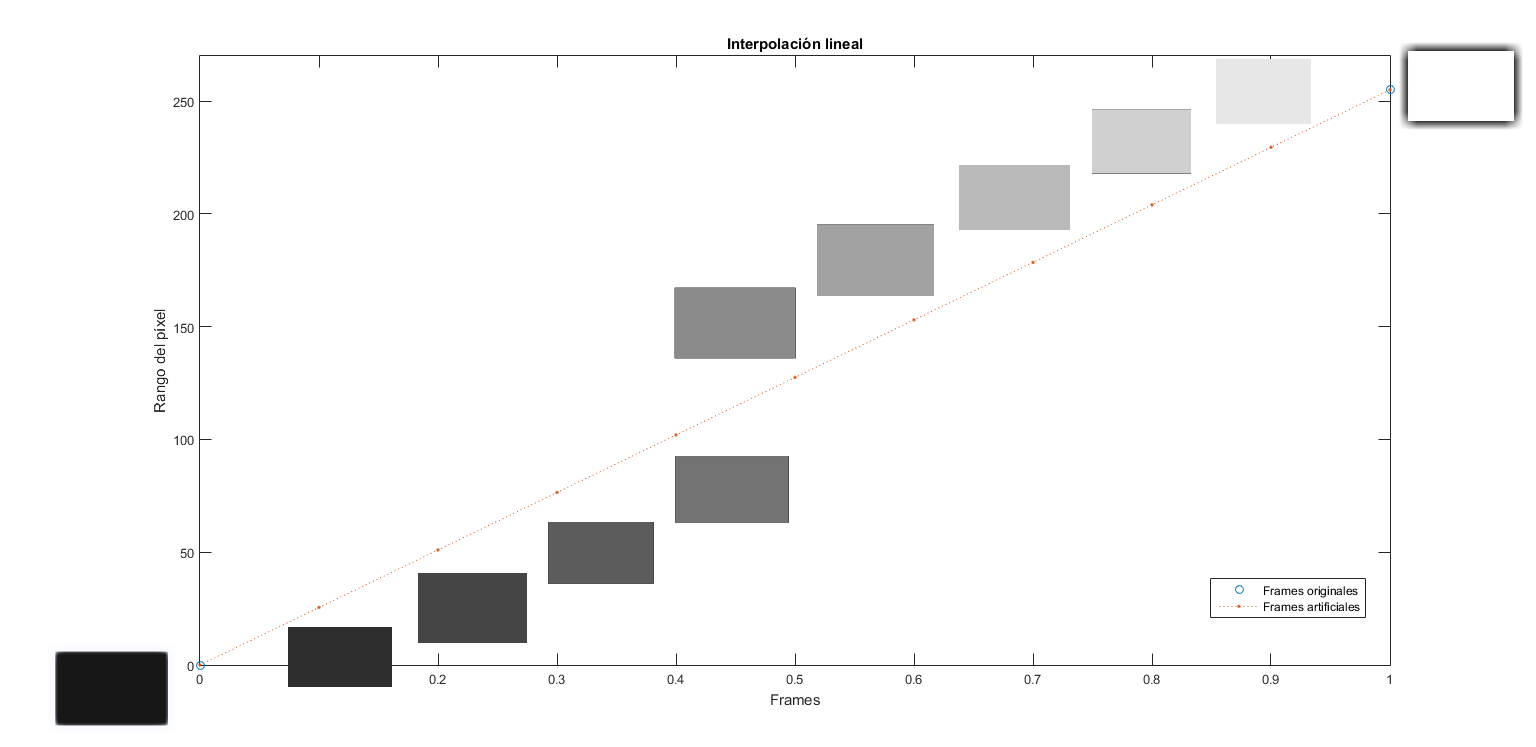
\includegraphics[width=0.75\textwidth]{GraficoLineal.png}
     \caption{Muestra del momento en que se realiza el cambio de blanco a negro, con sus respectivos frames intermedios}\label{fig:linealValidacion}
\end{figure}
\noindent

\subsubsection*{Splines}

Seguimos con la misma metodolog\'ia que con interpolaci\'on lineal, definiendo la funci\'on en cuesti\'on:

$f(x) = a (x - x0)^3 + b ( x - x0)^2 + c ( x - x0) + d$

Pero, ¿C\'omo hallamos los coeficientes del polinomio? Podr\'iamos por un lado, realizar las cuentas a papel y  de ah\'i seguir con el procedimiento de verificar con respecto a la implementaci\'on. Sin embargo, eso ser\'ia  bastante engorroso de realizar, por lo que optamos por usar un software inteligente cuyo nombre es $MatLab$. Usando la funci\'on $interpo1$ podemos obtener el valor de cualquier punto intermedio, en particular los que se evaluaron en nuestro programa.

No obstante, si bien al notar que efectivamente la funci\'on $f(x)$ se asemeja a una funci\'o lineal, hay que tener en cuenta una herramienta clave en $Splines$: la construcci\'on por bloques. Pero como decidimos que cada bloque comparta su primer y \'ultimo frame (excepto los extremos, que comparten alguno de los 2), luego no existe el caso de que se divida de forma tal que quede todo negro de un lado y blanco en lo que sigue.

\subsubsection*{\bf{Resultado:}}

Ideamos una instancia con par\'ametro de adici\'on de frames igual a 5, y dividido en 16 bloques. Como lo que importa aqu\'i es validaci\'on y no performance, optamos por un valor menor. Dicho esto, mediante $MatLab$ visualizamos cada Spline generado por bloque y comparando con la implementaci\'on, no se encontr\'o ninguna objeci\'on a lo ya comentado.

Con el gr\'afico \ref{fig:splineValidacion}, identificamos lo que $MatLab$ produjo al enviarle los puntos pertenecientes al bloque donde se hallaba el cambio de blanco a negro y de ah\'i, comparamos con los frames que obtuvimos.

\begin{figure}[h!]
  \centering
    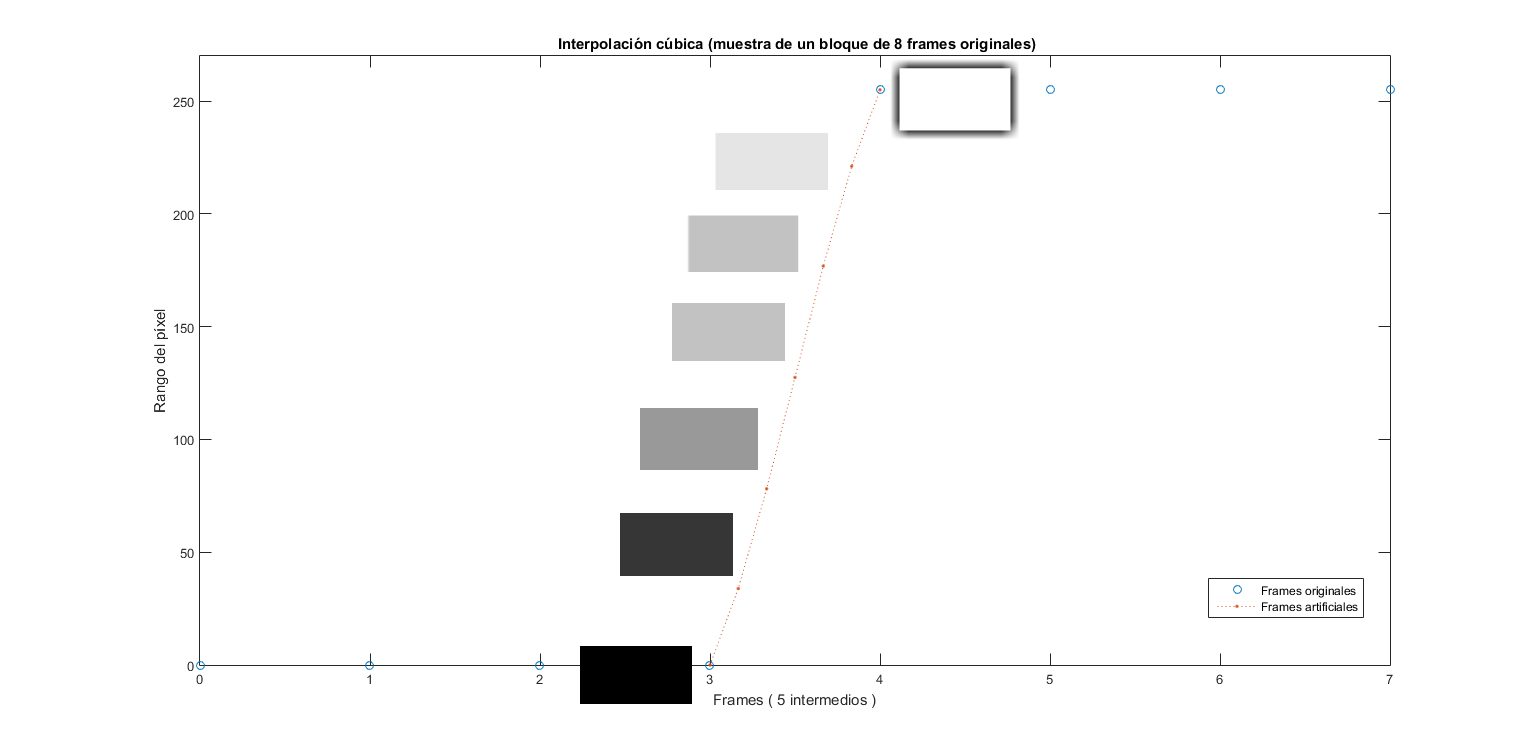
\includegraphics[width=0.75\textwidth]{GraficoSplines.png}
     \caption{Muestra del bloque que contiene el cambio, con los cuadros comparados}\label{fig:splineValidacion}
\end{figure}
\noindent

%---------------------------------------------------------------
\subsubsection{C\'amara Fija - Im\'agen Fija}

Equivalente a pensar que una im\'agen est\'a siendo reproducida durante un lapso de tiempo, que difiere al hecho de que una c\'amara est\'e quieta, enfocando a un objeto que puede ser sofocado por la luz. Y est\'a claro que el mero hecho de querer alentizar un video de tal caracter\'istica, solo servir\'a para aumentar la duraci\'on de la misma. Por lo conceptualmente visto, no hay dudas de que si la implementaci\'on se realiz\'o de forma correcta, no existir\'ia ning\'un cambio en el video.

Usamos metodolog\'ias id\'enticas para los tres m\'etodos. Esto es, extraer cada cuadro artificial y corroborar que coincide con la foto utilizada.

\subsubsection*{\bf{Resultado:}}

Como en cada p\'ixel $(i,j)$ el valor se mantuvo constante, as\'i lo fue con las funciones interpoladoras. De esta manera, cualquier punto que era evaluado por m\'as frames que se le quisiese acomodar, solo produc\'ia un video m\'as largo. En conclusi\'on, la im\'agen permeneci\'o intacta durante toda su reproducci\'on.


%---------------------------------------------------------------
\newpage
\subsection{Tiempos de ejecuci\'on}
\begin{figure}[h!]
  \centering
    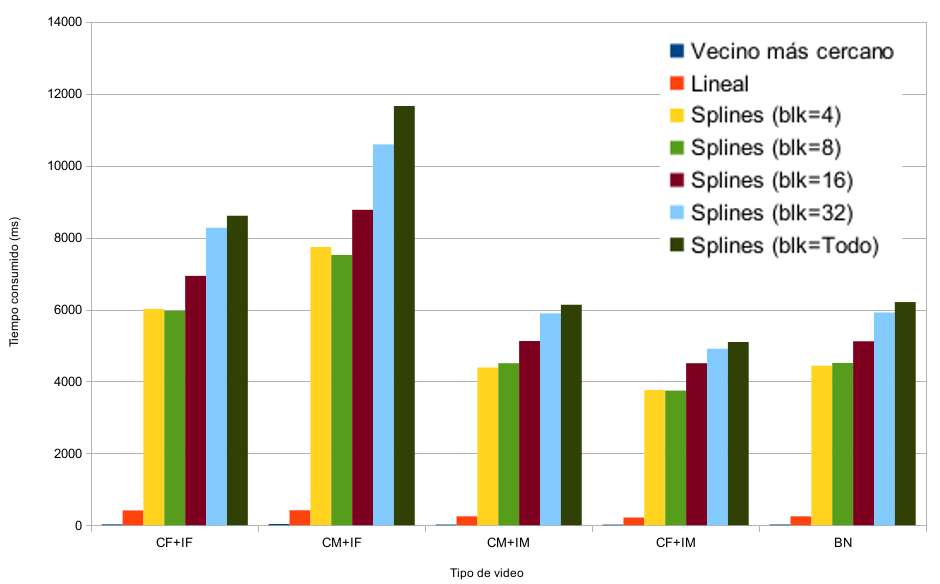
\includegraphics[width=\textwidth]{tiempos-tipo-video.png}
     \caption{Tiempo de ejecución de cada método por tipo de video}\label{fig:tiempos}
\end{figure}
\noindent


\begin{figure}[h!]
\centering
    \subfloat[][Por tipo de video, para videos de ``laboratorio'']{
        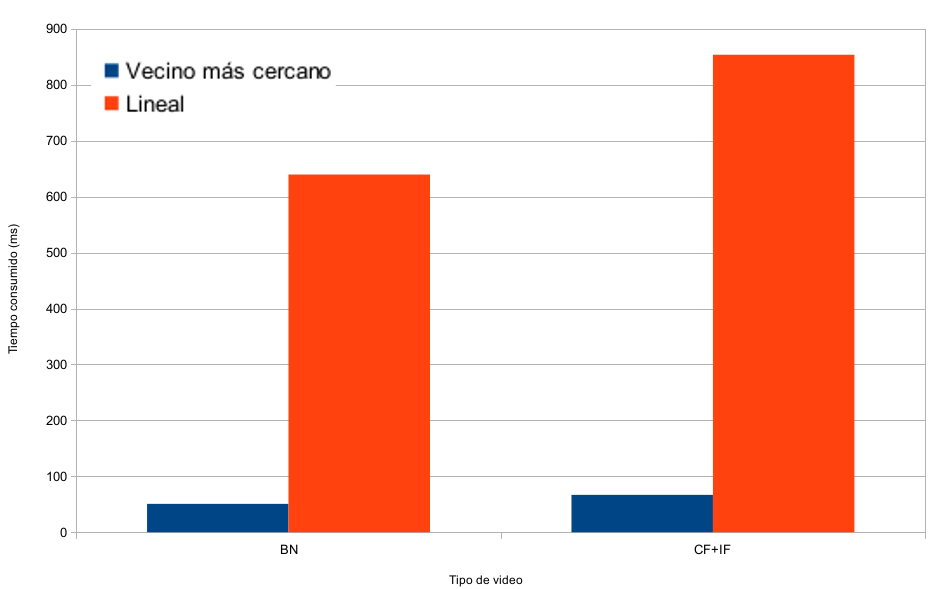
\includegraphics[width=0.5\textwidth]{tiempos-laboratorio.png}
        \label{fig:tiempos-lab}
    }
    \subfloat[][Por cantidad de frames del video]{
        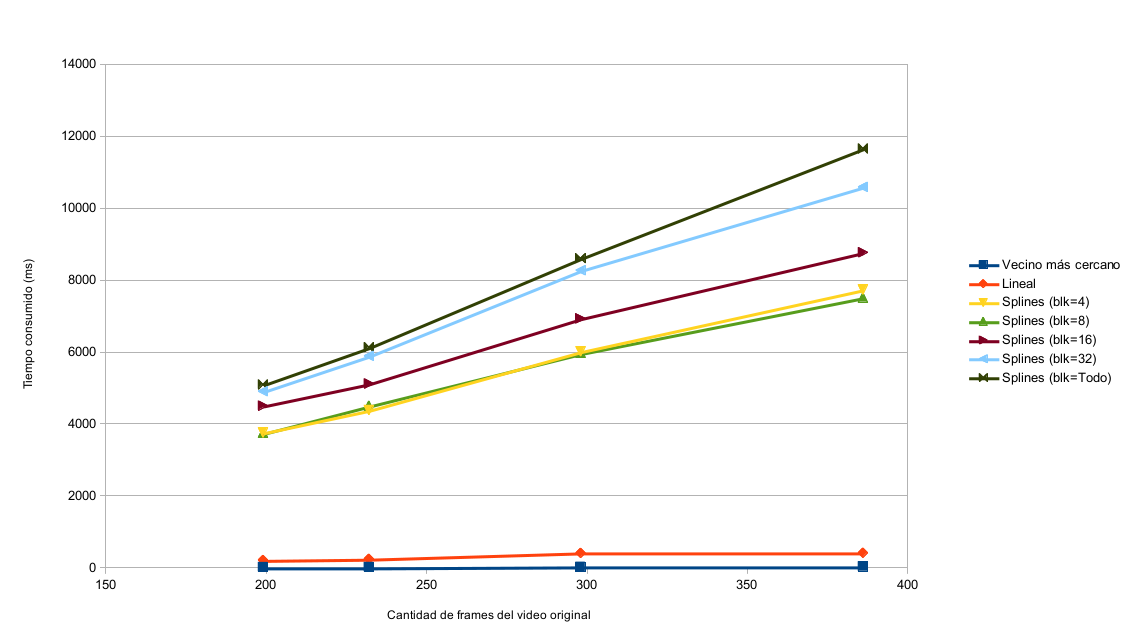
\includegraphics[width=0.5\textwidth]{tiempos-cant-frames.png}
        \label{fig:tiempos-cant-frames}
    }
    \caption{Tiempo de ejecuci\'on de cada M\'etodo}
\end{figure}

Al medir los tiempos de los métodos para cada tipo de video utilizado, fijando en 10 la cantidad de frames a agregar, obtuvimos lo graficado en la figura \ref{fig:tiempos}. Puede apreciarse claramente, como podía adivinarse, que el método de interpolación por splines tarda mucho más que los demás, mientras que el método de vecino más cercano toma tiempos casi imperceptibles, menores a 30ms para cualquier tipo de video.

Un resultado notable es que, para la interpolación por splines, la relación entre el tamaño de los bloques de frames y el tiempo consumido no resultan proporcionales. Esto puede explicarse con el hecho de que, si bien un tamaño de bloque menor implica que los sistemas de ecuaciones sean menores, también hace que sean más sistemas. Y viceversa: a mayor tamaño de bloque, menos bloques hay y por lo tanto menos sistemas hay que resolver. Según observamos en nuestros experimentos, el tamaño de bloque necesario para obtener la mejor perfomance oscila entre 4 y 8 frames, dependiendo del tipo de video.

De modo similar, observamos que tomar el video completo como un único bloque no es mucho peor que considerar bloques de tamaño 32 frames (al menos no con los videos que utilizamos, de pocos segundos). Asociamos esto al hecho de que, en ese caso, hace falta resolver un único sistema de ecuaciones.

Para los dos métodos más rápidos, realizamos el mismo experimento para nuestros videos de ``laboratorio'': el pasaje de negro a blanco y la foto fija convertida en un video constante. En la figura \ref{fig:tiempos-lab} pueden observarse los resultados, donde nuevamente se confirma que el método de Vecino más cercano es hasta un orden de magnitud más rápido que el de Interpolación lineal.

Finalmente, realizamos la comparación del tiempo consumido por cada método y la cantidad de frames del video original. Los resultados pueden verse en la figura \ref{fig:tiempos-cant-frames}. De su observación notamos que el costo de ejecutar los métodos parece depender linealmente de la cantidad de frames del video, y que la pendiente parece ser más fuerte para los splines que para los demás métodos. Dentro de los splines, vemos que la pendiente varía para bloques de tamaño 4 y 8, pero que para tamaños de bloque mayores, la pendiente aumenta cuando aumenta el tamaño de bloque.


%---------------------------------------------------------------
\newpage
\subsection{C\'amara Fija - Im\'agen Fija}\label{subsec:fija-fija}
\IEEEPARstart{E}{n} principio podría parecerle al lector que este experimento
carece de sentido, por estar evaluando un video que no tiene
movimiento de ning\'un tipo. Aunque esto no es estrictamente cierto: en el caso evaluado, se tiene
un video de la vista de unos edificioes y la transici\'on del d\'ia a la noche.
Esto hace que cambien las \emph{tonalidades} o brillo de las distintas partes del video.

As\'i pues, un caso que en principio har\'ia pensar ``la
interpolaci\'on deber\'ia funcionar sin error pues no hay movimiento''
(como se mencion\'o en la validación) no resulta tan evidente.

Comenzamos entonces a presentar los resultados obtenidos a partir de la
aplicaci\'on de los m\'etodos explicados e implementados para este video.

%---------------------------------------------------------------
\subsubsection{Spline}\label{subsubsec:fija-fija_spline}
\par Lo primero a tener en cuenta al experimentar con este m\'etodo es que
tenemos 2 variables (la tercera variable, el video, est\'a fija): la cantidad
de frames a interpolar y el tama\~no de bloque. Decidimos entonces, primero
``fijar'' la cantidad de frames a interpolar y an\'alizar que ocurre al variar
el tama\~no del bloque.

\begin{figure}[H]
    \centering
    \subfloat[][ECM para 10 frames interpolados]{
        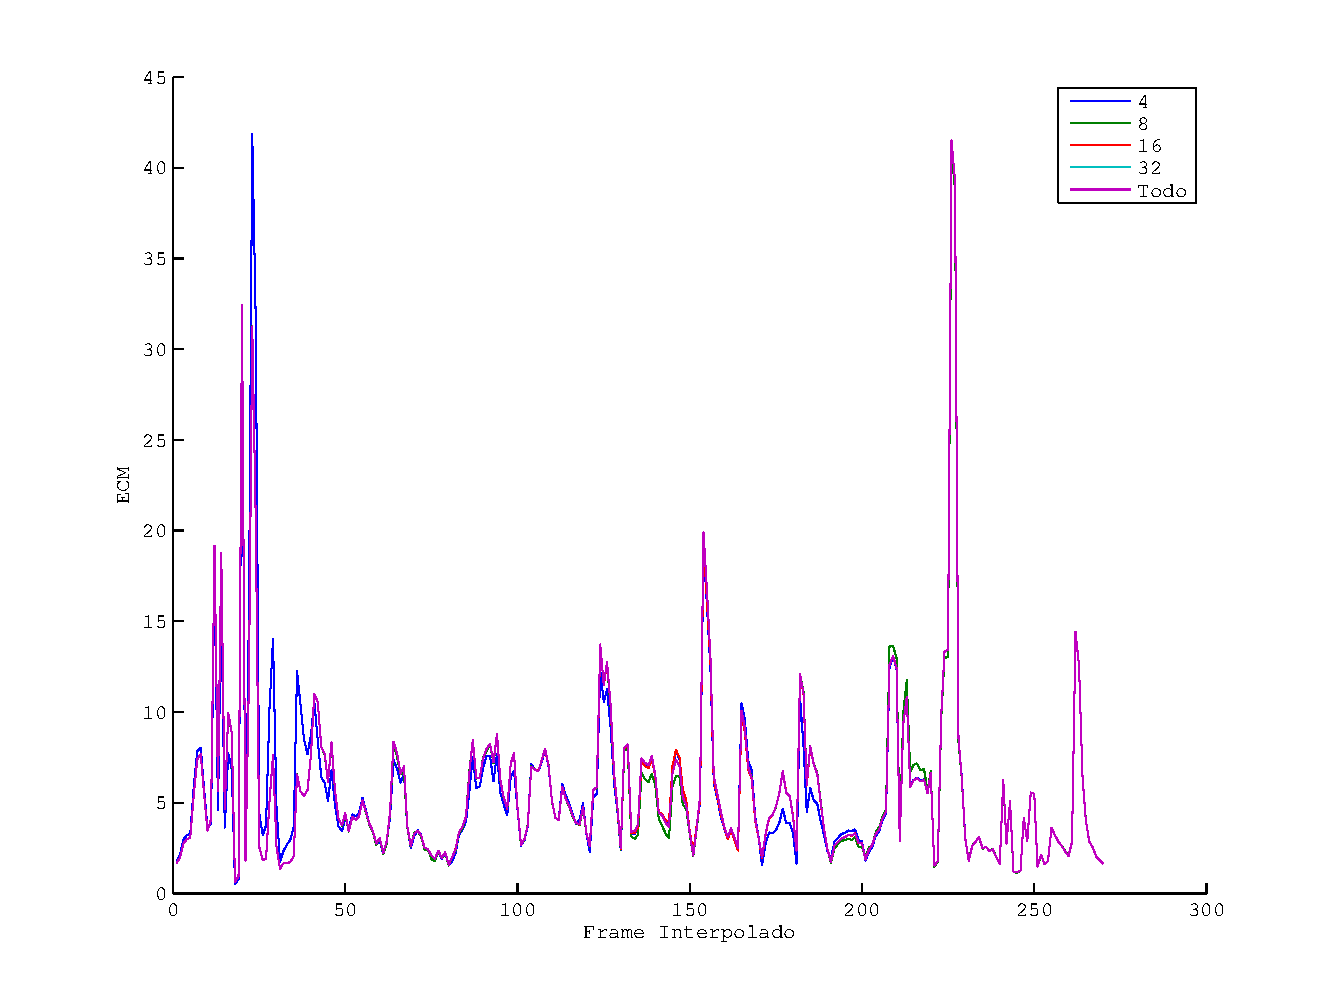
\includegraphics[width=.5\textwidth]{mse_spline-camara_fija-imagen_fija-k10.pdf}
        \label{subfig:fija-fija_spline-mse-k10}
    }
    \subfloat[][PSNR para 10 frames interpolados]{
        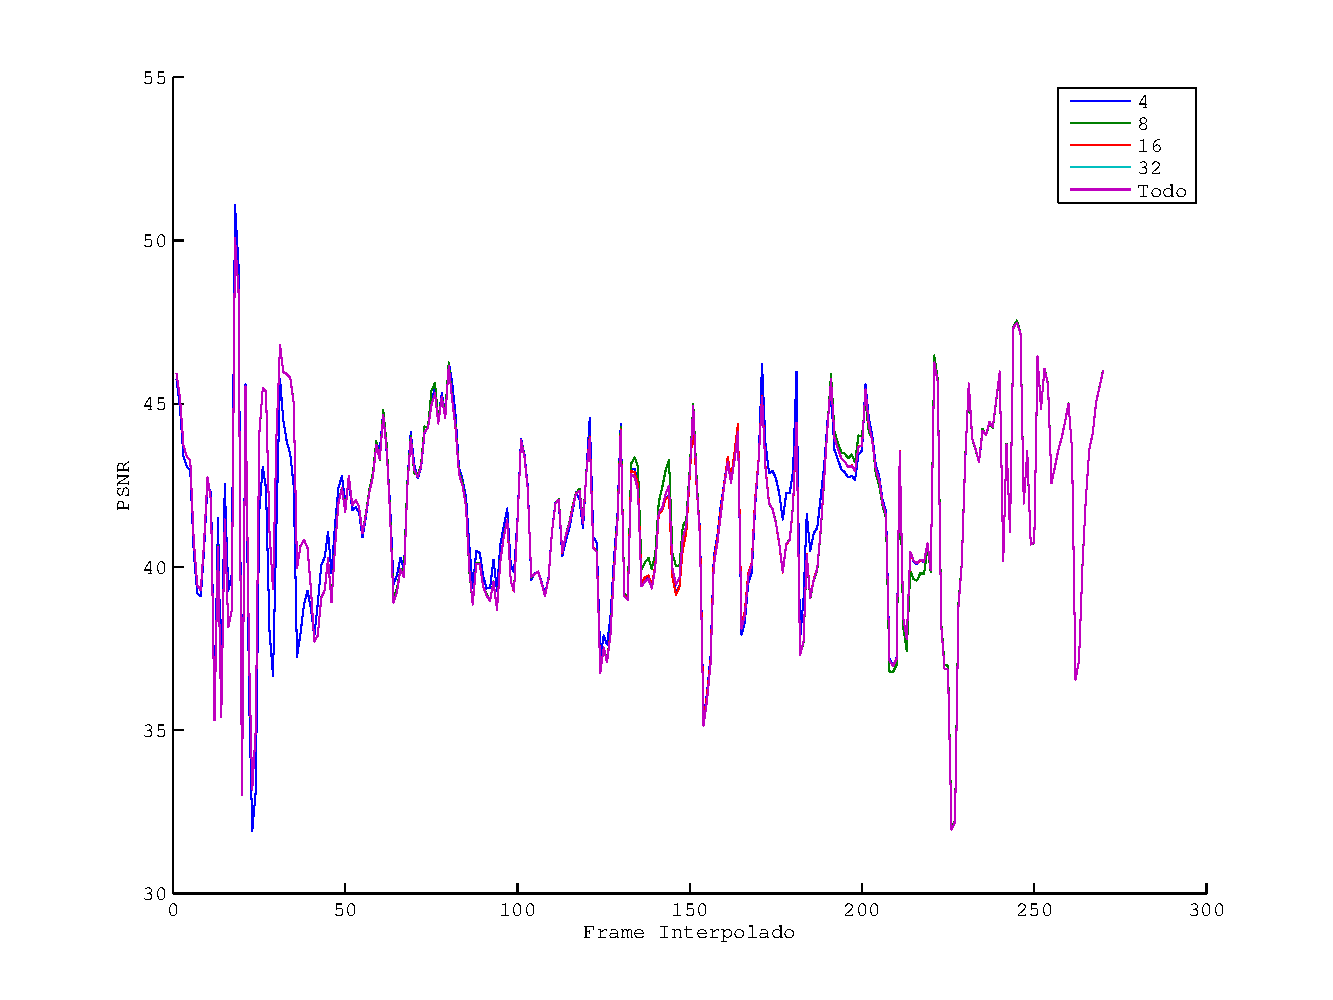
\includegraphics[width=.5\textwidth]{psnr_spline-camara_fija-imagen_fija-k10.pdf}
        \label{subfig:fija-fija_spline-psnr-k10}
    }
    \caption{Comparativa tama\~no de bloque para 10 frames interpolados}
    \label{fig:fija-fija_spline-bloques}
\end{figure}

\par Se puede observar en la figura \ref{fig:fija-fija_spline-bloques} que las
m\'etricas utilizadas (ECM y PSNR) para los distintos tama\~nos de bloques son
pr\'acticamente id\'enticas: est\'an solapadas casi igual para todos los frames
interpolados del video. Si bien en los gr\'aficos expuestos se pueden llegar a
notar ciertas regiones de frames donde alguno de los tam\~nos de bloque difiere
(por ejemplo, en la figura \ref{subfig:fija-fija_spline-mse-k10} en el bloque de
frames del 1 al 50 se ve que para el tama\~no de bloque 4 tenemos 2 picos: uno
donde tiene un mayor ECM que el resto y otro donde tiene un menor ECM, lo cual
se ve reflejado tambi\'en en la gr\'afica del PSNR\footnote{D\'onde para el pico
de mayor ECM se obtiene un PSNR menor que el resto, y al rev\'es para el pico de
menor ECM. Esto tiene sentido ya que como se explic\'o, el PSNR es una m\'etrica
de la calidad de la interpolaci\'on/estimaci\'on del frame, y tener un mayor
ECM indica menor calidad en la estimaci\'on.}), como comportamiento general
observamos que el tama\~no del bloque (aplicado ''a ciegas'' sobre la totalidad
del video) no nos asegura una mejor ni peor estimaci\'on/interpolaci\'on. Este
patr\'on se repite para las restantes variantes en funci\'on de la cantidad
de frames interpolados, motivo por el cual s\'olo exponemos los resultados para
$10$ frames interpolados a la hora de describir este comportamiento.

\par Habiendo analizado que el tama\~no del bloque (utilizado de la manera
explicada) no pareciera tener influencia en el error comentido en un sentido
amplio (ya que observamos como var\'ia el ECM y PSNR frame a frame), evaluamos
algunos resultados m\'as ''estad\'isticos'', si se quiere, del ECM a lo largo
de todos los frames seg\'un cada tama\~no de bloque.

\begin{figure}[H]
    \centering
    \subfloat[][Valor medio, Desv\'io Est\'andar, M\'aximo y M\'inimo\label{tbl:spline_k10}]{
        \footnotesize
        \setlength{\tabcolsep}{3pt}
        \begin{tabular}{|l|r|r|r|r|}
            \hline
            \textbf{Bloque}& \textbf{Mean}& \textbf{Std}& \textbf{M\'ax}& \textbf{M\'in}\\
            \hline\hline
            4& 5.6919& 5.4221& 41.8650& 0.5080\\
            8& 5.6497& 5.0825& 40.8340& 0.6403\\
            16& 5.6812& 5.0828& 41.5168& 0.6407\\
            32& 5.6881& 5.0950& 41.5173& 0.6407\\
            Entero& 5.6881& 5.0950& 41.5173& 0.6407\\
            \hline
        \end{tabular}
    }\hspace{10pt}
    \subfloat[][Diferencia M\'axima\label{tbl:dif_spline_k10}]{
        \footnotesize
        \setlength{\tabcolsep}{3pt}
        \begin{tabular}{|l|r|r|r|r|r|}
            \hline
            \textbf{Bloque}& \textbf{vs 4}& \textbf{vs 8}& \textbf{vs 16}& \textbf{vs 32}& \textbf{vs Entero}\\
            \hline\hline
            \textbf{4}& 0& 11.0099& 11.0156& 11.0156& 11.0156\\
            \textbf{8}& 2.9723& 0&  1.0059&  1.0069&  1.0069\\
            \textbf{16}& 2.8873&  1.4356& 0&  0.5544&  0.5544\\
            \textbf{32}& 2.9104&  0.9827&  0.6176& 0& 0\\
            \textbf{Entero}& 2.9104&  0.9827&  0.6176& 0& 0\\
            \hline
        \end{tabular}
    }
    \caption{Comparativa ECM seg\'un tama\~no de bloque}
\end{figure}

\par Si observamos la tabla \ref{tbl:spline_k10}, obsevamos resultados que
validan lo observado previamente: el tama\~no del bloque no pareciera influir
en el error cometido. Las diferencias son m\'inimas, salvo por ah\'i el error
m\'inimo cometido por el tama\~no de bloque 4 es menor que para los dem\'as
tama\~nos de bloque y que su desv\'io est\'andar es un poco mayor. Aunque estas
diferencias tambi\'en son muy peque\~nas, siendo despreciables a la hora de
afirmar que el tama\~no de bloque no afecta al error cometido.

\par Continuando, si se observa la tabla \ref{tbl:dif_spline_k10}, la cual nos
se\~nala la diferencia m\'axima de los errores cometida entre dos interpolaciones
con distinto tama\~no de bloque (es decir, cual fue la diferencia m\'as amplia
del ECM para un mismo frame entre dos tama\~nos de bloque), observamos que
el tama\~no de bloque 4 cometi\'o, respecto de los dem\'as tama\~nos, un error
m\'as amplio que los dem\'as. Si volvemos a observar la figura
\ref{subfig:fija-fija_spline-mse-k10}, podemos observar que hay un claro pico
de error m\'as alto para el tama\~no de bloque 4 entre los primeros 50 frames.
Seguramente esta diferencia observada en la tabla se debe a dicho frame, donde
el tama\~no de bloque 4 cometi\'o mucho m\'as error que los dem\'as m\'etodos.
Descartando este valor, conclu\'imos que el tama\~no de bloque no afecta (salvo
casos aislados) al error cometido por la interpolaci\'on mediante
spline\footnote{Por cuestiones de tiempo no se pudo buscar exactamente el frame
donde ocurri\'o esta \'ultima diferencia explicada, para observar su
correlaci\'on con lo que ocurre en el video.}.

\par Hasta ahora hemos analizado lo que ocurre para diferentes tama\~nos de
bloque. Pasamos entonces a observar que ocurre para diferentes cantidades de
frames interpolados.

\begin{figure}[H]
    \centering
    \subfloat[][ECM para 1 frame interpolado]{
        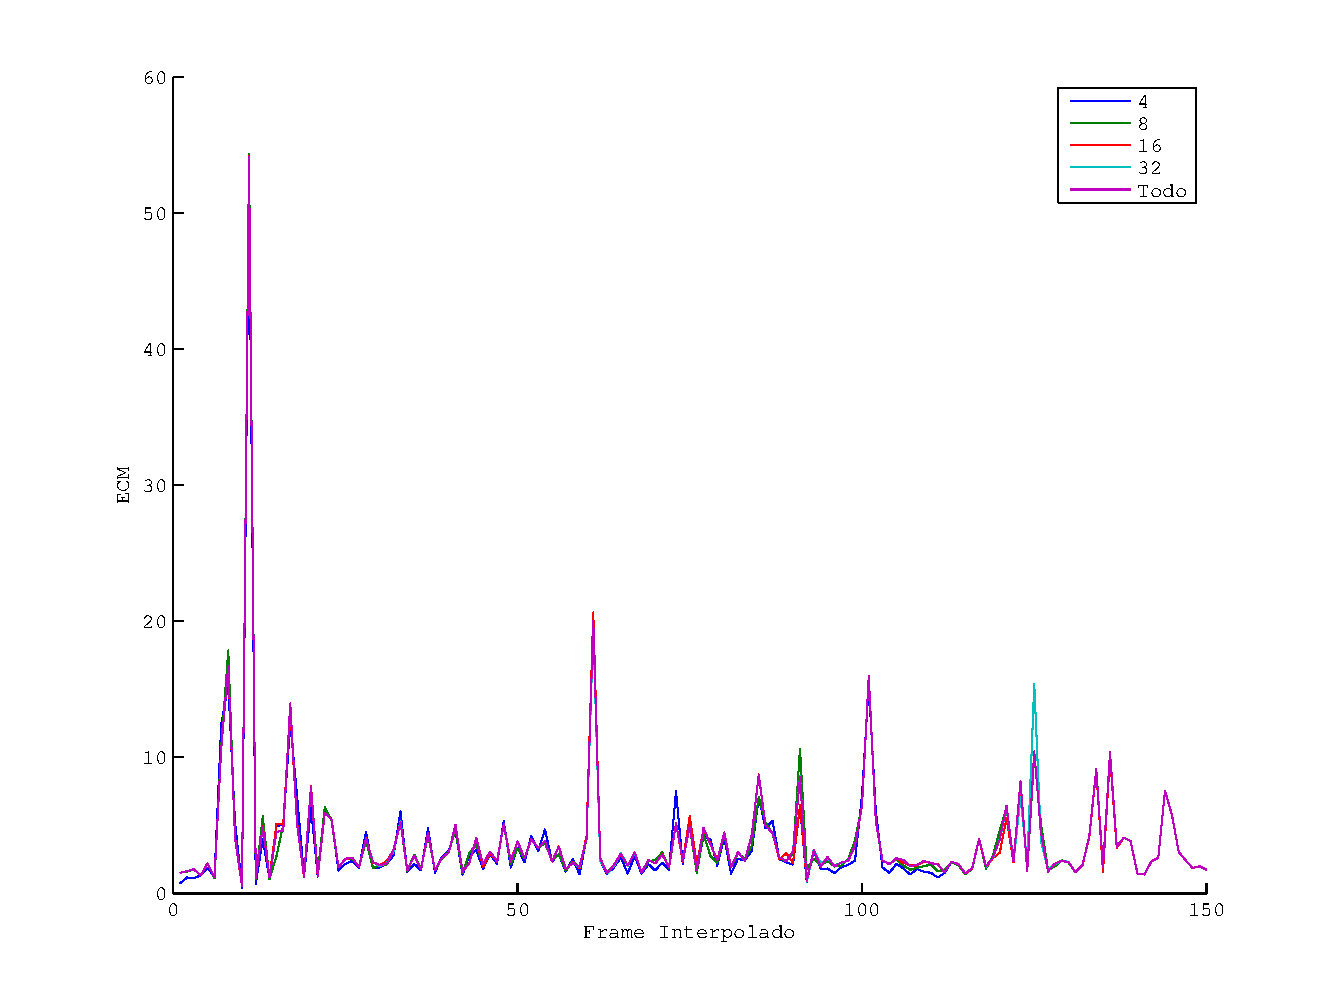
\includegraphics[width=.5\textwidth]{mse_spline-camara_fija-imagen_fija-k1.pdf}
        \label{subfig:fija-fija_spline-mse-k1}
    }
    \subfloat[][ECM para 5 frames interpolados]{
        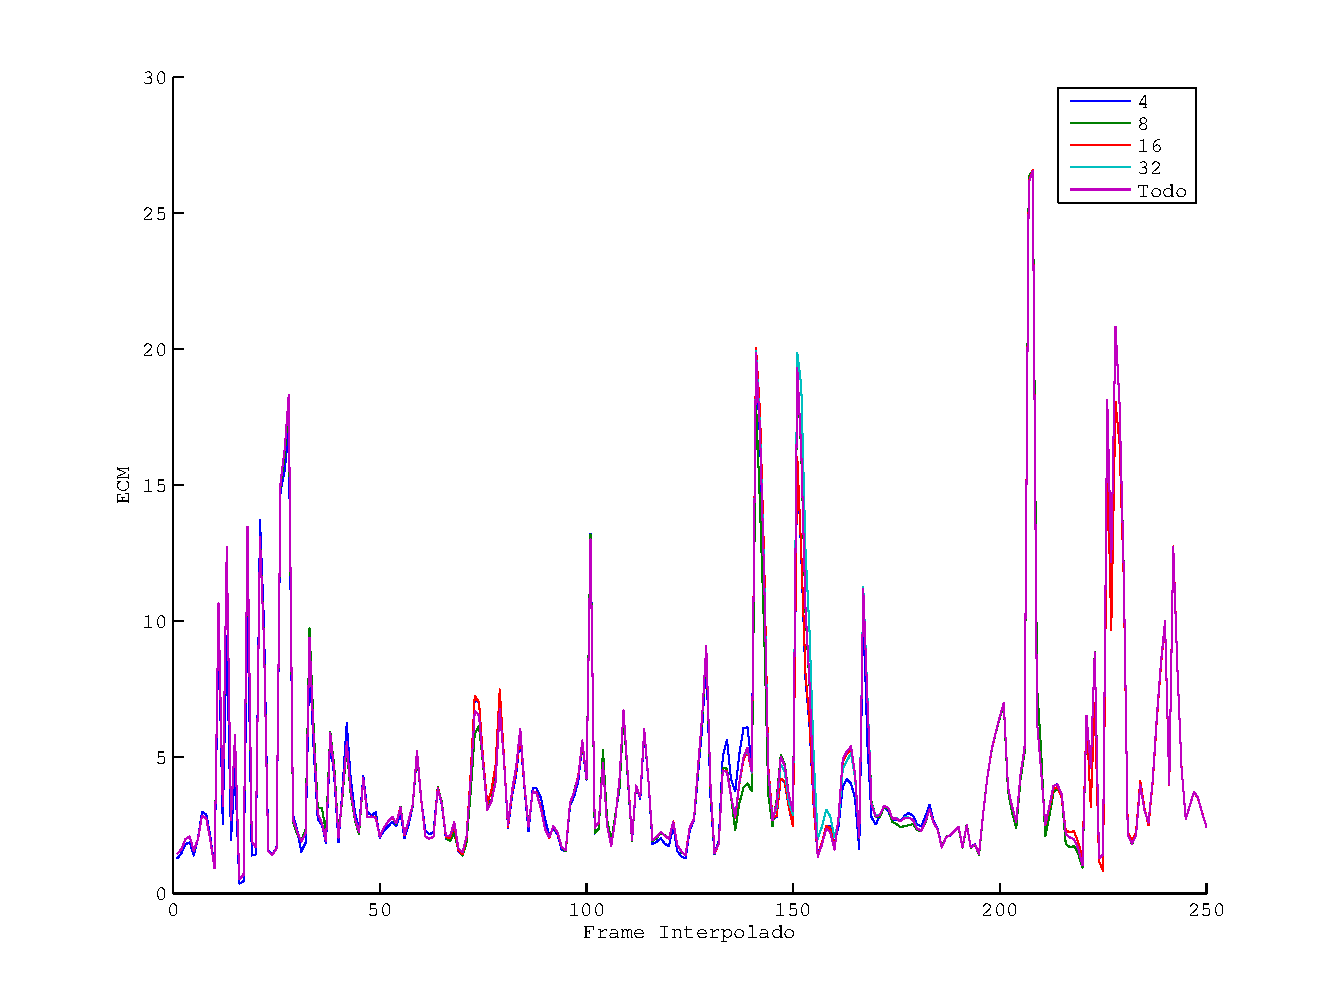
\includegraphics[width=.5\textwidth]{mse_spline-camara_fija-imagen_fija-k5.pdf}
        \label{subfig:fija-fija_spline-mse-k5}
    }
    \caption{Comparativa seg\'un cantidad de bloques interpolados}
    \label{fig:fija-fija_spline-frames-interpolados}
\end{figure}

\par Lo primero, evidente, que salta a la vista de observar las figuras
\ref{subfig:fija-fija_spline-mse-k10}, \ref{subfig:fija-fija_spline-mse-k1} y
\ref{subfig:fija-fija_spline-mse-k5}, es la cantidad (y valor o intensidad) de
los picos de error. Se ve que a medida que se incrementa la cantidad de frames
interpolados, comienzan a acentuarse el comportamiento en ''picos'' de los
errores frame a frame, siendo cada vez m\'as amplia la diferencia entre el
m\'inimo error cometido de un ''pico'' y el error m\'aximo alcanzado en el mismo
(observar con detenimiento la escala de las figuras). A su vez se observa de
manera intuitiva que la media del ECM ir\'ia aumentando a medida que se interpolan
cada vez m\'as frames. Esto \'ultimo tiene sentido, ya que ahora se tienen frames
cada vez m\'as distantes y se interpolan todos los frames intermedios. A mayor
distancia entre los frames ''dato'' que se usan para calcular el polinomio
interpolador, se puede pensar que menos informaci\'on se tiene y por lo tanto
la calidad de la estimaci\'on se ve perjudicada.

\par Por otra parte, se observa un comportamiento similar, aunque de distinta
intensidad, en los 3 gr\'aficos: el ECM tiene un comportamiento oscilante,
aunque no c\'iclico ni constante. Es decir, se ve que el ECM tienede a
incrementarse hasta llegara un ''pico'', para luego comenzar a descender. Y
as\'i repetidamente (pero, como se a dicho, la ''intensidad'', o valores que
alcanza -tanto m\'inimos como m\'aximos locales- var\'ia a lo largo de los
frames del video). Prestando una mayor atenci\'on, se nota que el ECM tiende a
ser m\'as bajo para aquellos frames que est\'an m\'as cerca de alguno de los
frames originales (no interpolados) del video. Nuevamente, el valor m\'aximo
del ECM alcanzado para los frames contenidos entre 2 frames originales/no
interpolados var\'ia (todav\'ia por motivos desconocidos), pero el
comportamiento de incrementarse el ECM a medida que nos alejamos de un frame
original y decrementarse al acercarse es un patr\'on que se da en todos los
casos.

\par Observermos los datos est\'adisticos del ECM para los diferentes valores
de los frames interpolados\footnote{Estos datos solo consideran los frames
interpolados}:

\begin{figure}[H]
    \centering
    \subfloat[][Valor Medio]{
        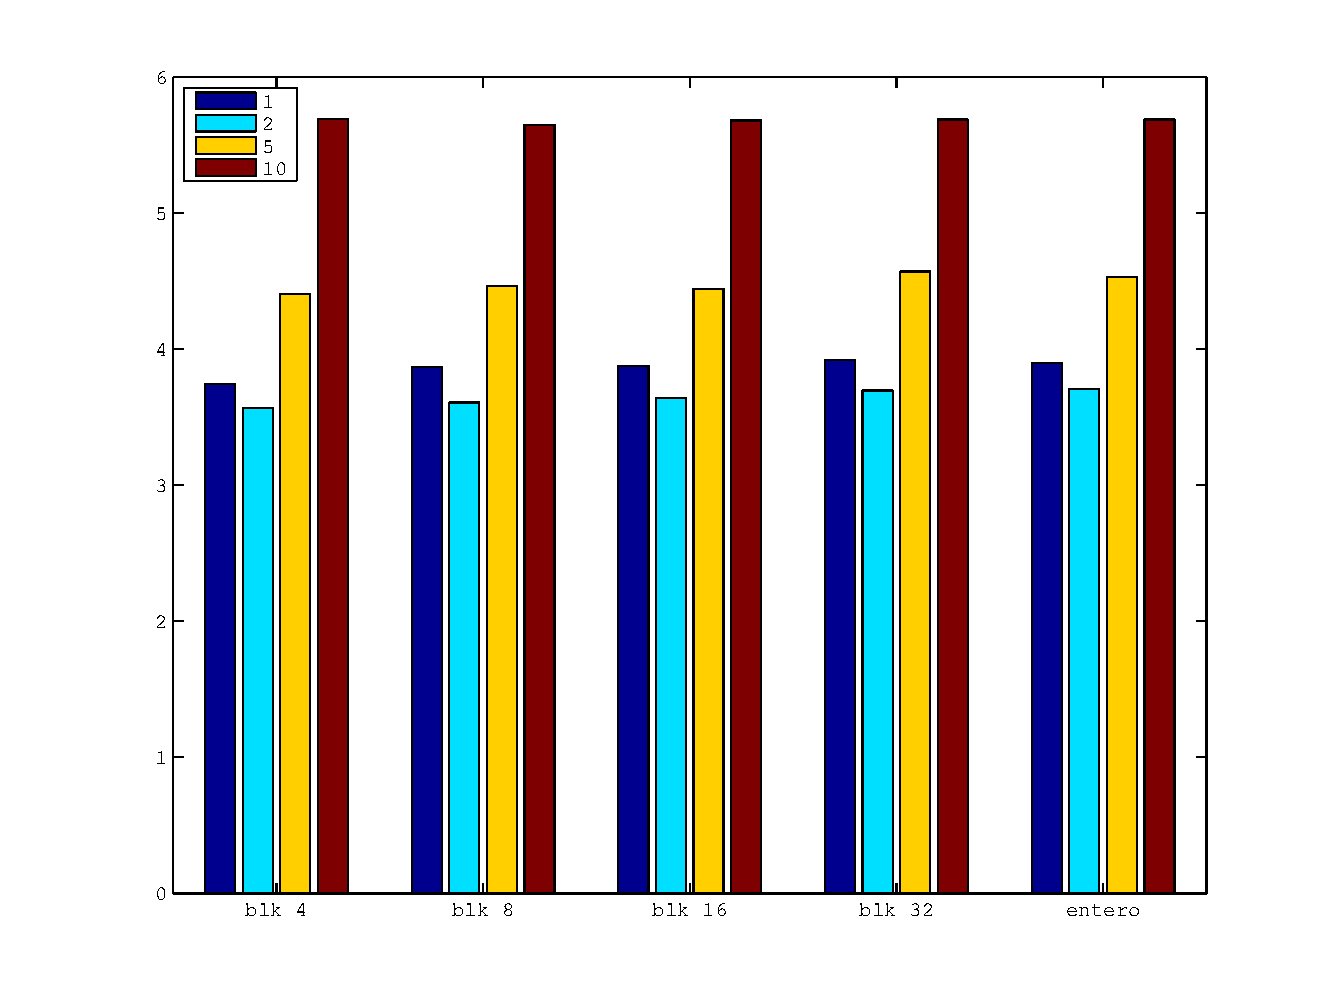
\includegraphics[width=.5\textwidth]{camara_fija-imagen_fija-mean_spline.pdf}
    }
    \subfloat[][Desv\'io Est\'andar]{
        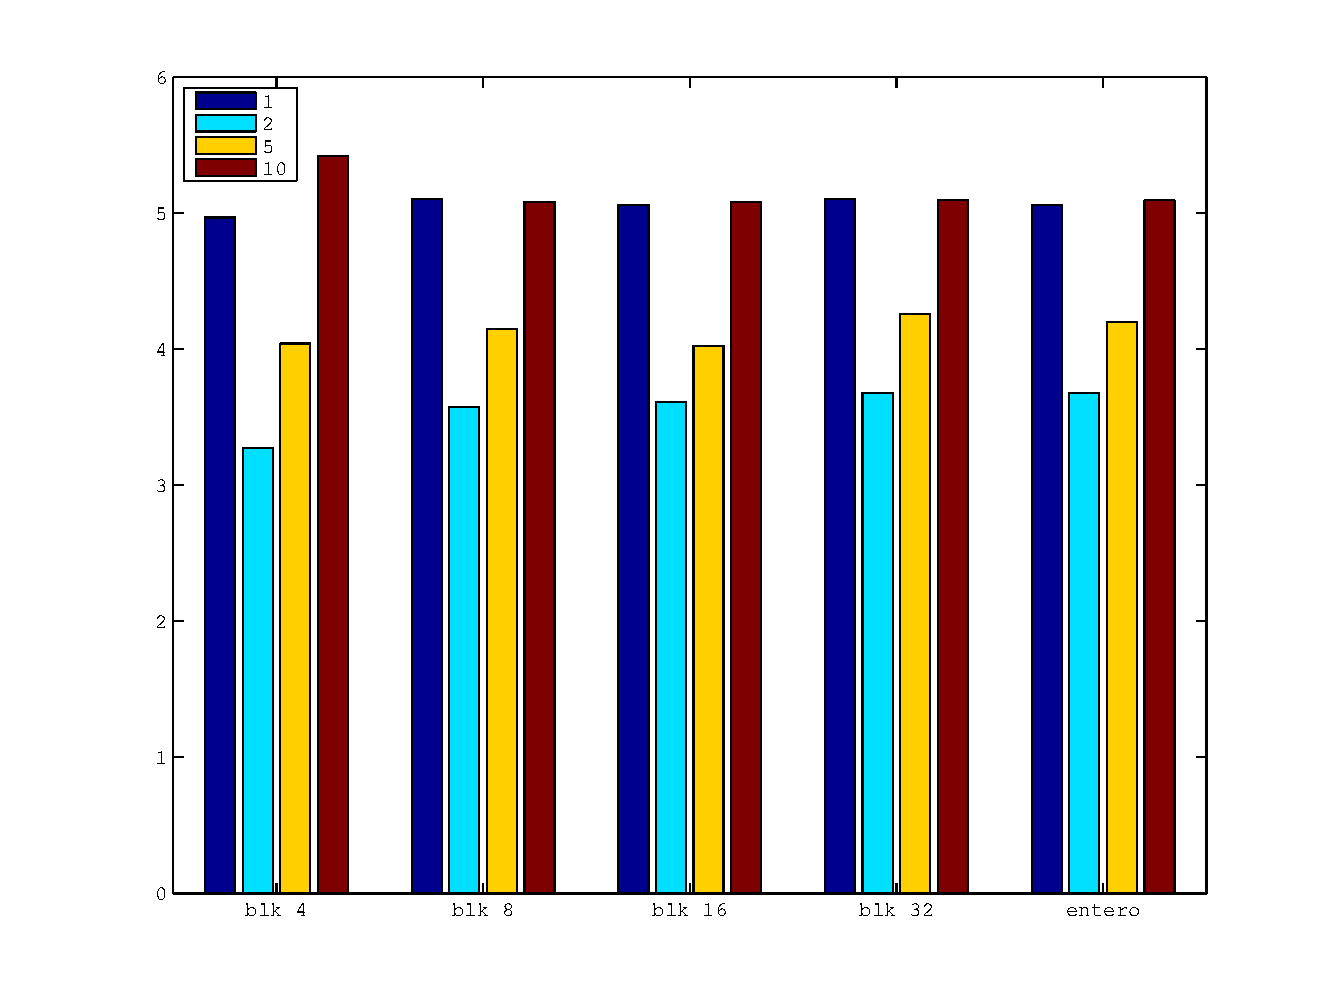
\includegraphics[width=.5\textwidth]{camara_fija-imagen_fija-std_spline.pdf}
    }\\
    \subfloat[][M\'aximo]{
        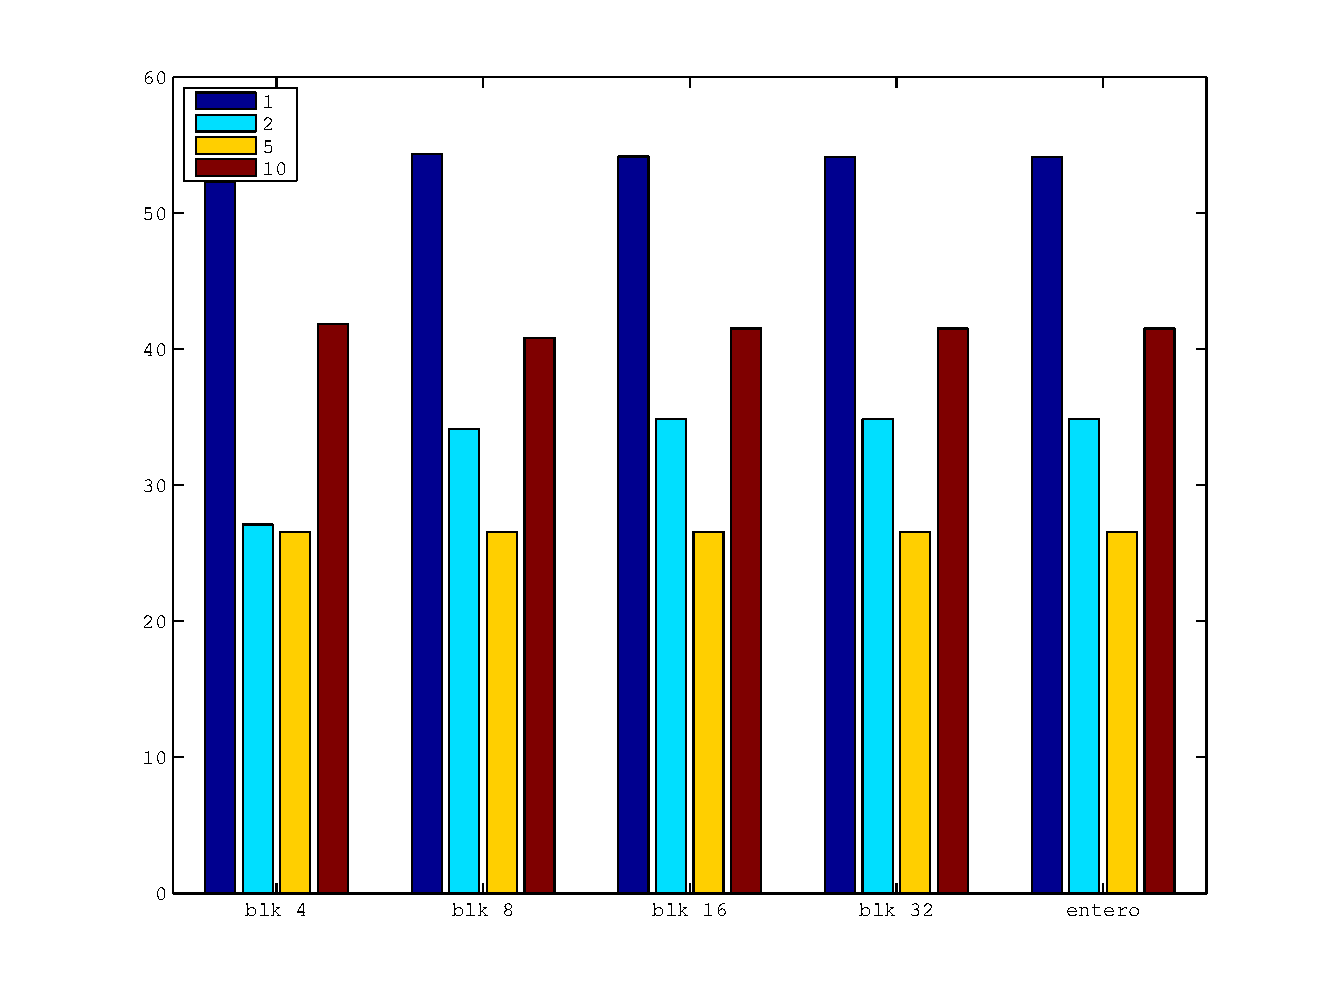
\includegraphics[width=.5\textwidth]{camara_fija-imagen_fija-max_spline.pdf}
    }
    \subfloat[][M\'inimo]{
        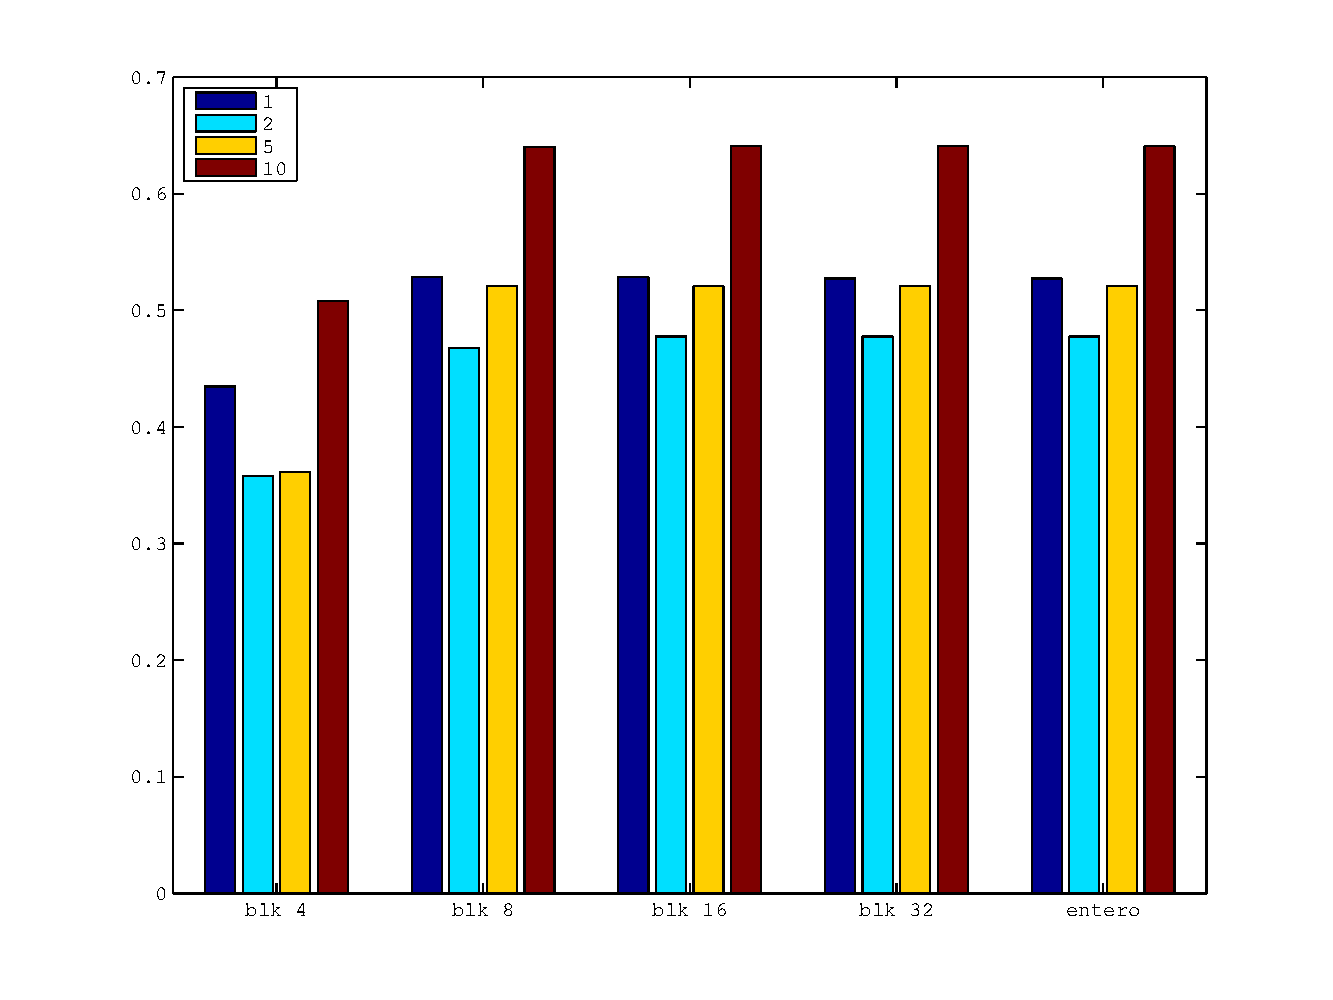
\includegraphics[width=.5\textwidth]{camara_fija-imagen_fija-min_spline.pdf}
    }
    \caption{Est\'adisticas ECM Seg\'un Frames Interpolados - Spline}
    \label{fig:fija-fija_spline-mse_estadisticas}
\end{figure}

\par Analizando la figura \ref{fig:fija-fija_spline-mse_estadisticas}, lo primero
que salta a la vista es que claramente hay un patr\'on en el ECM comparando por
tama\~no de bloques. La relaci\'on entre los distintos valores de frames
interpolados se mantiene para cada grupo correspondiente al tama\~no de bloque.
Esto es consistente con los resultados vistos anteriormente en esta misma
secci\'on.

\par En segundo lugar, ya concentrandonos en la cantidad de frames interpolados,
vemos un resultado que no era esperado seg\'un nuestras hip\'otesis: observamos
un valor medio de error, desv\'io est\'andar y error m\'aximo que es notoriamente
menor para la interpolacio de 2 frames (e incluso, se obtuvo la mejor
aproximaci\'on de un \'unico frame, como se observa en el gr\'afico del ECM
m\'inimo). Es decir, pare este video observamos que se obtienen los mejores
valores generales de error cuando se interpola de a 2 frames en lugar de a 1,
como se plante\'o en las hip\'otesis. Pareciese que para este video, tener un
poco menos de informaci\'on mejora sustancialmente el ECM (ver la comparaci\'on
para 1 frame versus 2 frames).

\par Siguiendo esta misma l\'inea de an\'alisis, observamos al interpolar 1 frame
y 10 nos dan un desv\'io est\'andar alto comparado con las interpolaciones de 2
y 5 frames, aunque los valores medios del error para 10 frames son muchos m\'as
altos que para el resto de los valores. Esto \'ultimo si confirma, parcialmente,
la hip\'otesis de que a mayor cantidad de frames interpolados, mayor ser\'a el
error (o peor la aproximaci\'on).

\par Para finalizar el an\'alisis de estos datos, resulta realmente sorpresivo
observar un error medio menor para la interpolaci\'on de 2 frames que para la
de 1 frame. A\'un as\'i, la diferencia entre estos es m\'inima, y si
despreciamos esta diferencia diciendo que la diferencia es tan peque\~na que
podemos considerar que ambas tiene el mismo ECM medio, vemos confirmada la
hip\'otesis ya mencionada, ya que a mayor cantidad de frames interpolados,
mayor error medio. Aunque vale la pena mencionar que, el desv\'io est\'andar
nos indica que para una interpolaci\'on de 1 frame en este tipo de videos,
tenemos una gran varianza frame a frame de la calidad de la interpolaci\'on.
Descontando este valor sorpresivo, observamos que esta varianza mantiene la
relaci\'on inicialmente esperada, aumentando a medida que aumenta la cantidad
de frames interpolados.

\par Por \'ultimo, es interesante tratar de asociar los errores cometidos por
el m\'etodo con lo que est\'a ocurriendo en el video. En la figura
\ref{fig:fija-fija_spline-heatmap} se puede observar una captura del video
comparativo de este m\'etodo para tama\~no de bloque 4 y cantidad de frames
interpolados 1\footnote{\url{https://drive.google.com/open?id=0B0RfkWV-4-XqNFJMT1l5NXg2VHM}}.

\par Decidimos utilizar estos par\'ametros ya que de los datos vistos
previamente, con los mimos tenemos un valor alto (relativo a los dem\'as
par\'ametros) de varianza en el ECM frame a frame. De esta manera, consideramos
que ser\'ia menos costoso identificar la regi\'on (o regiones) del video que
m\'as influyen en el error de la interpolaci\'on.

\begin{figure}[H]
    \centering
    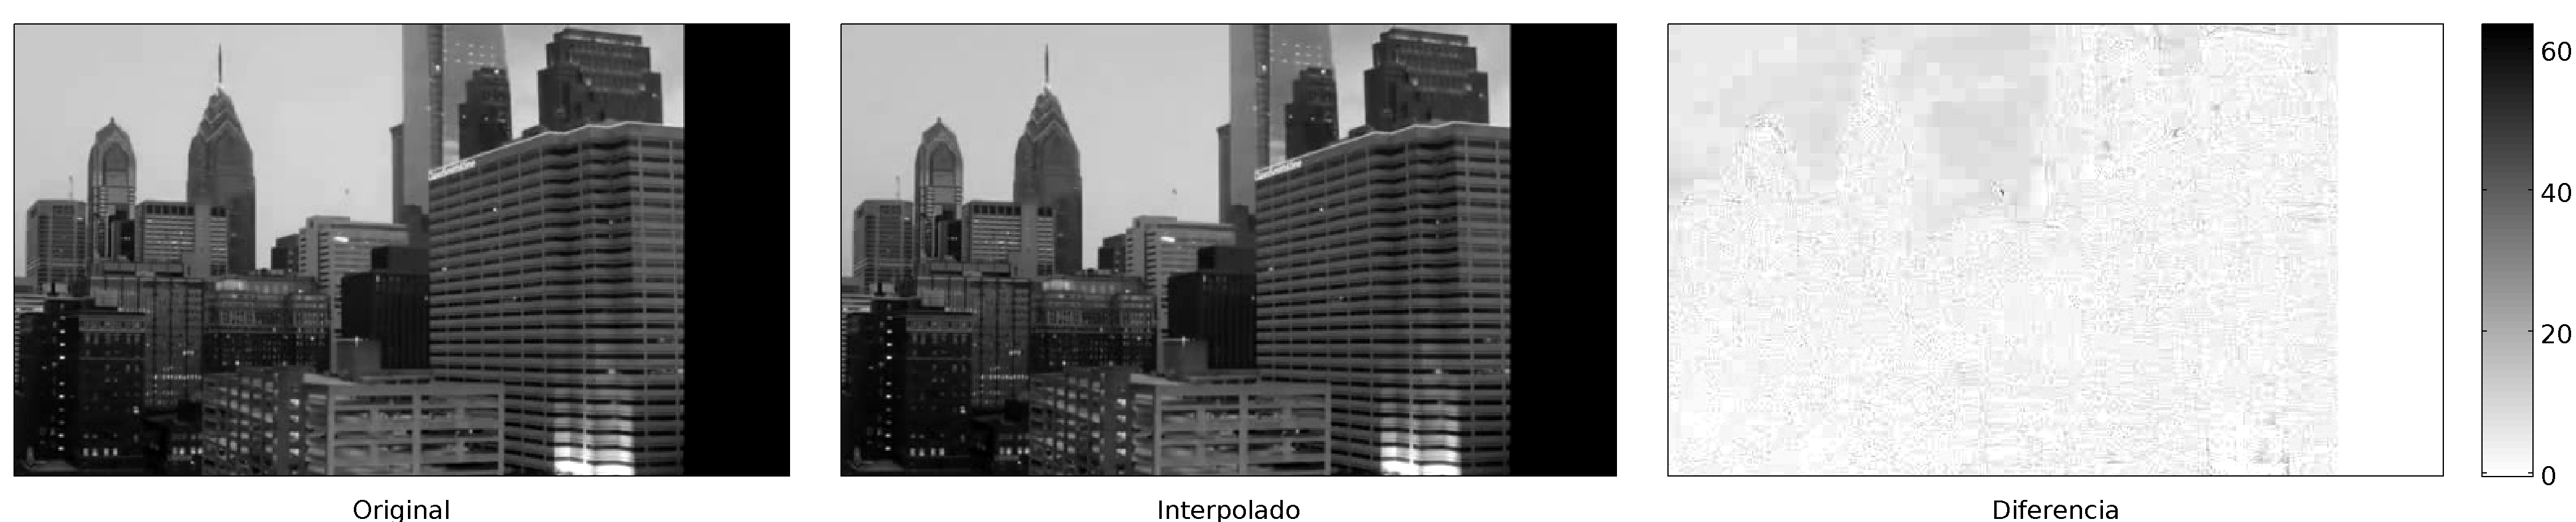
\includegraphics[width=\textwidth]{camara_fija-imagen_fija-spline-k1-blk4.png}
    \label{fig:fija-fija_spline-heatmap}
    \caption{Regi\'on peor aproximada por la interpolaci\'on por spline}
\end{figure}

\par En dicho video observamos que los pixeles que hacen al ECM est\'an
distribu\'idos por todo el frame, asociados seg\'un interpretamos, a los
cambios de iluminaci\'on\footnote{Recordemos que el video trata de unos
edificios (y parte del cielo) en una transici\'on acelerada del d\'ia a la
noche.}. La captura no es capaz de mostrar esto, pero la mostramos ya que es
representativa de la zona del video que es peor aproximada por la
interpolaci\'on. Se puede observar que aquellas partes m\'as afectadas por los
cambios de iluminaci\'on (el cielo y las partes altas de los edificioes) tienen
un error un poco m\'as alto que las partes bajas de los edificios
(especialmente la parte inferior izquierda), sobre las cuales el efecto de la
sombra de los dem\'as edificios mitiga el efecto de los cambios de
iluminaci\'on (ya que permanecen m\'as oscuros de por s\'i).

\par Es decir, se observa que aquellas partes del video que se ven m\'as
afectadas por cambios m\'as ''bruscos'' o diferenciados de iluminaci\'on (pasar
de alto brillo a poco brillo) son aquellas zonas que m\'as contribuyen al error
de la interpolaci\'on.

%---------------------------------------------------------------
\subsubsection{Interpolaci\'on Lineal}
\par A la hora de analizar los resultados de un mismos m\'etodo para distintos
valores de frames interpolados (como en toda esta secci\'on, la variable del
video se encuentra fijada), observar frame a frame y comparar el ECM/PSNR no
resulta un par\'ametro v\'alido. Esto se debe a que comprar cualquiera de estas
m\'etricas tiene sentido al hacerlo sobre un mismo frame interpolado, y dado que
para cada par\'ametro se interpolan distintos frames, la comparaci\'on carece
de sentido\footnote{Se podr\'ia tratar de encontrar frames interpolados en
com\'un, pero dicho trabajo complicaba mucho la tarea del an\'alisis y por
cuestiones de tiempo no pudo ser considerada esta opci\'on.}.

\par As\'i pues, a la hora de analizar y comprar un mismo m\'etodo y que ocurre
al tener que interpolar m\'as informaci\'on/frames, recurrimos a las m\'etricas
estad\'isticas del ECM que fueron presentadas en la experimentaci\'on anterior.
Las mismas pueden observarse en la figura
\ref{fig:fija-fija_lineal-mse_estadisticas}.

\begin{figure}[H]
    \centering
    \subfloat[][Valor Medio]{
        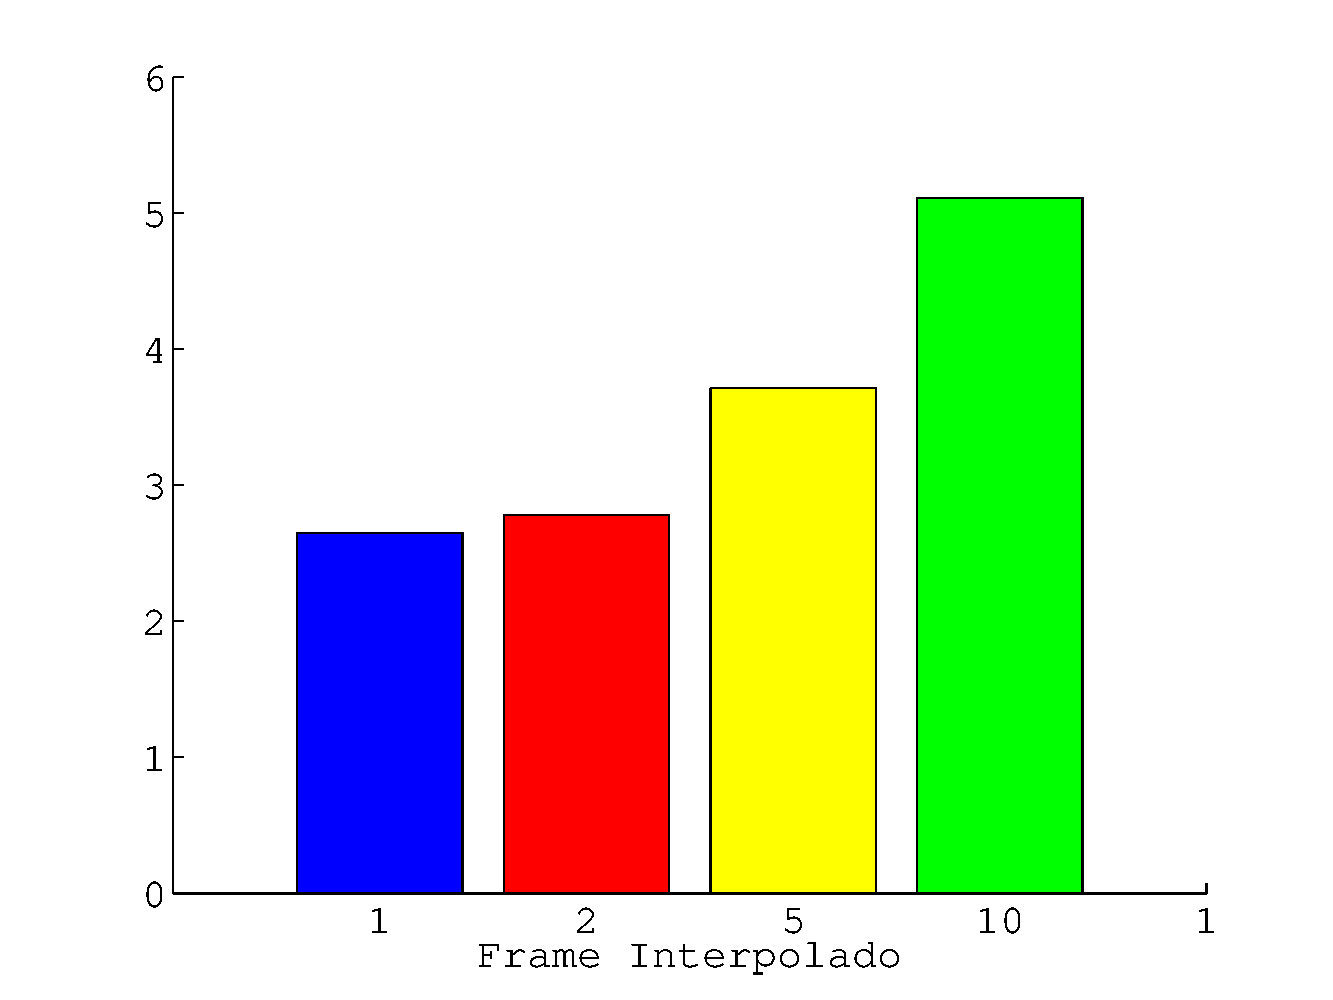
\includegraphics[width=.25\textwidth]{camara_fija-imagen_fija-mean_lineal.pdf}
    }
    \subfloat[][Desv\'io Est\'andar]{
        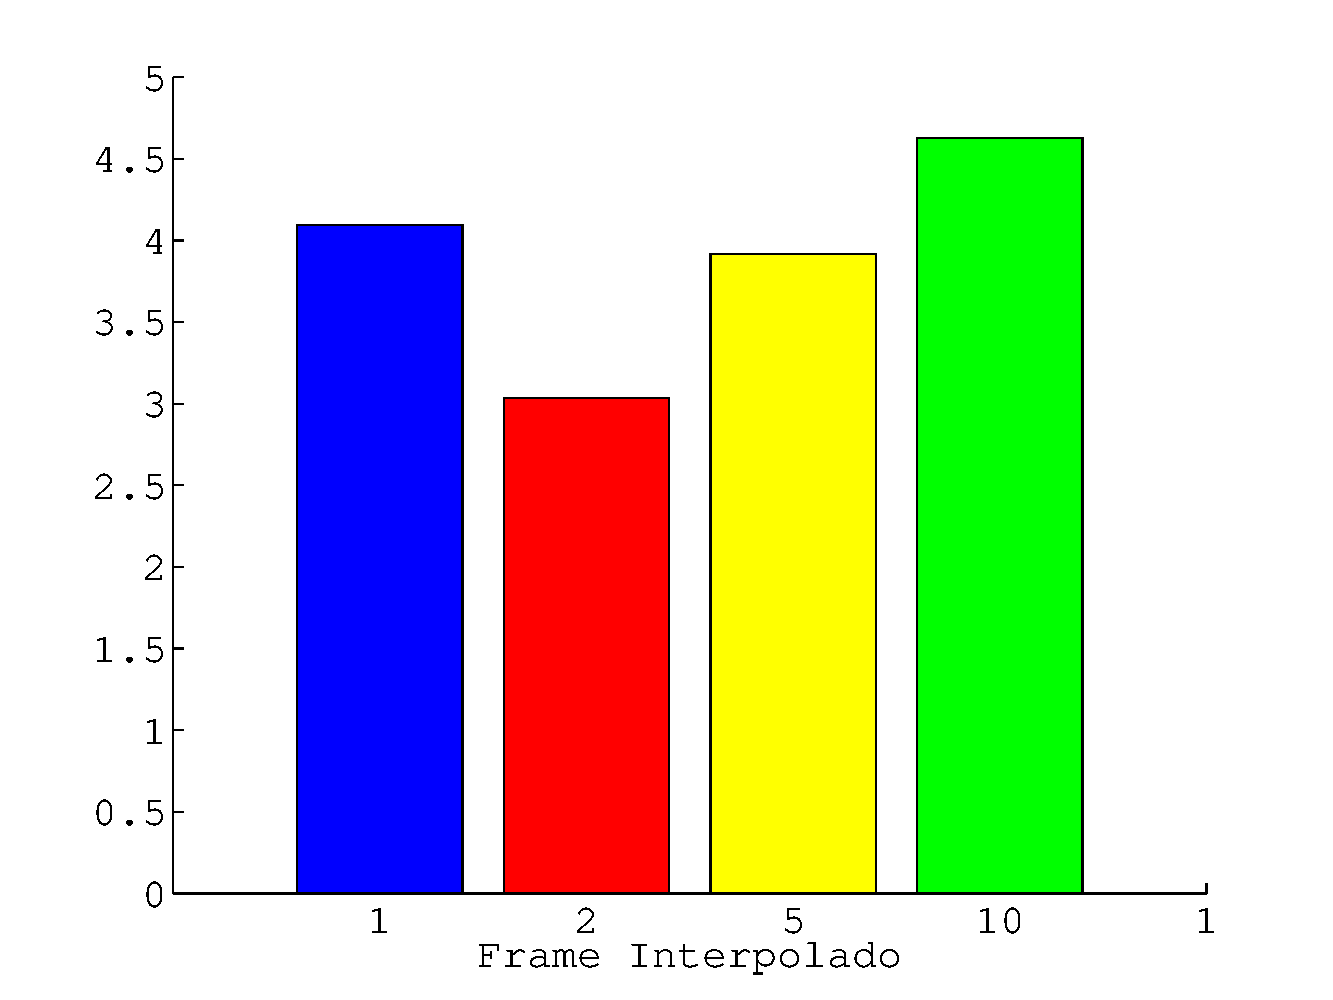
\includegraphics[width=.25\textwidth]{camara_fija-imagen_fija-std_lineal.pdf}
    }
    \subfloat[][M\'aximo]{
        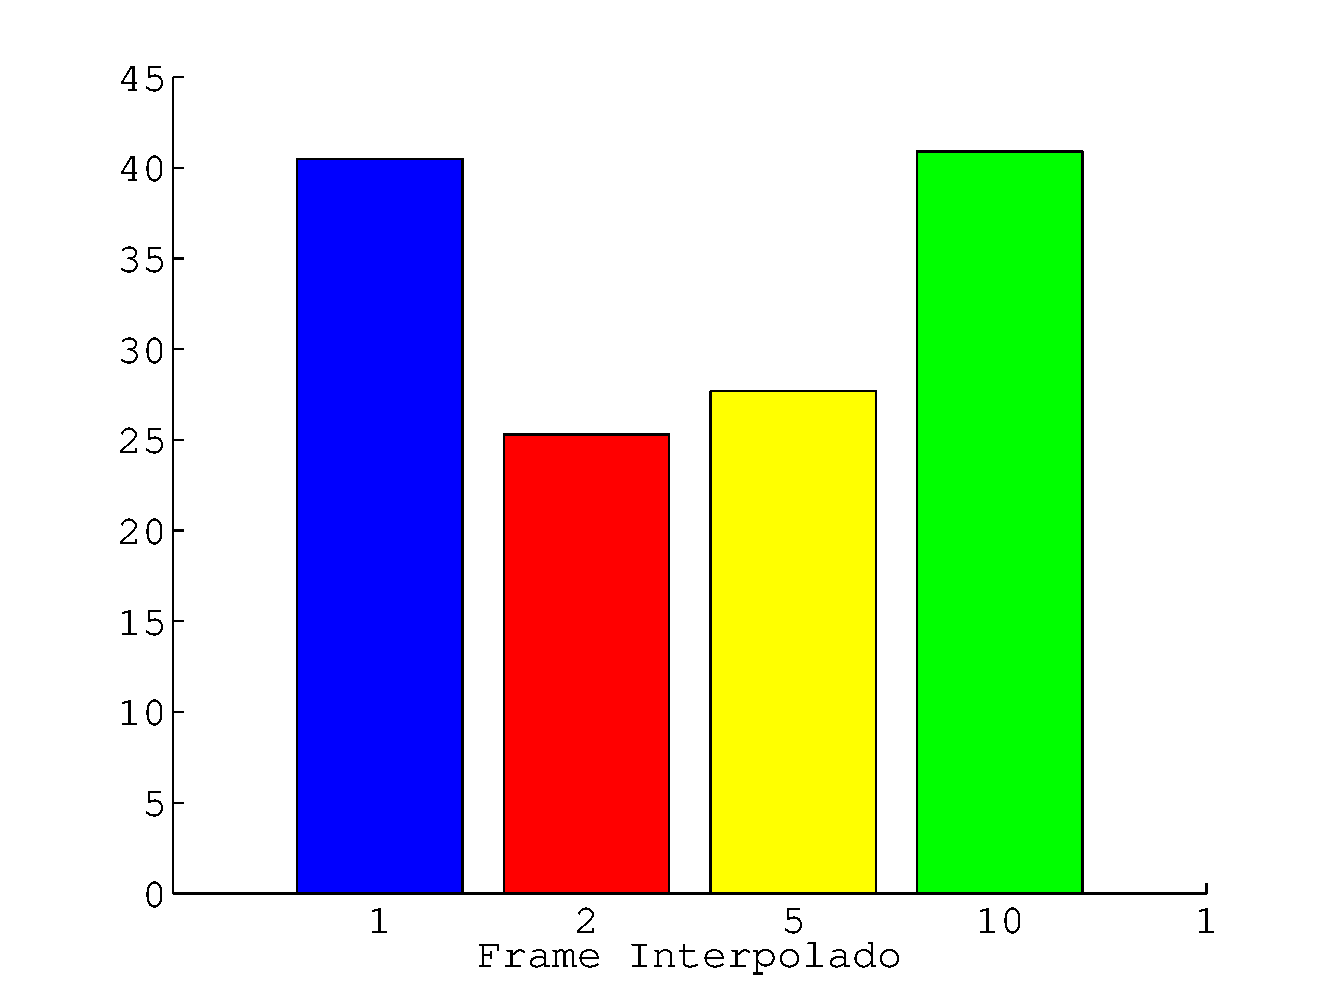
\includegraphics[width=.25\textwidth]{camara_fija-imagen_fija-max_lineal.pdf}
    }
    \subfloat[][M\'inimo]{
        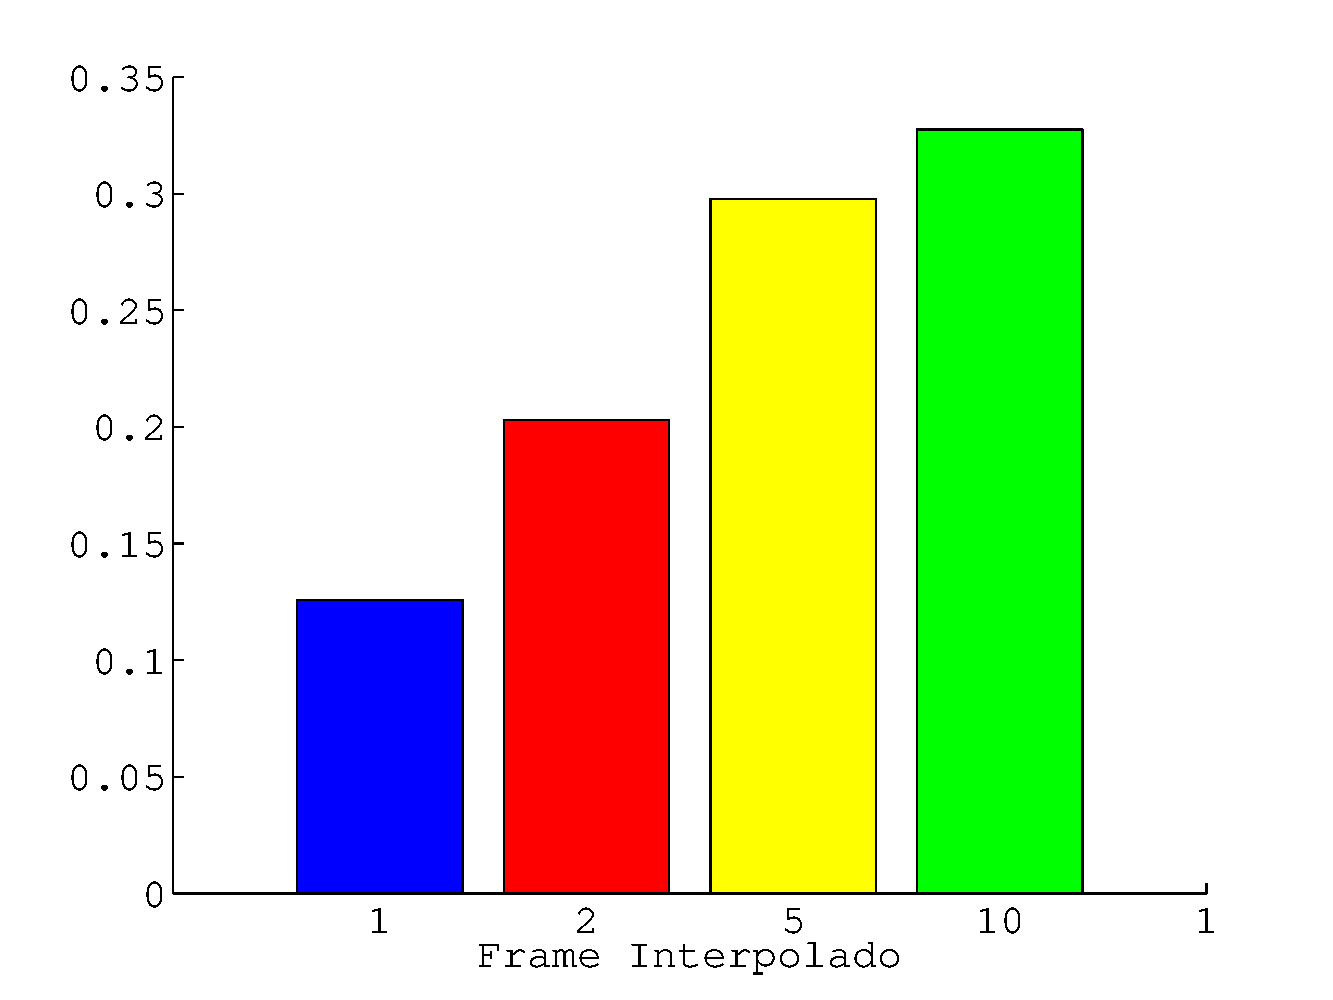
\includegraphics[width=.25\textwidth]{camara_fija-imagen_fija-min_lineal.pdf}
    }
    \caption{Est\'adisticas ECM Seg\'un Frames Interpolados - M\'etodo Lineal}
    \label{fig:fija-fija_lineal-mse_estadisticas}
\end{figure}

\par En este caso, como se puede observar en los gr\'aficos, nuestra
hip\'otesis sobre la calidad de la interpolaci\'on en funci\'on de la cantidad
de frames a interpolar se cumple para el valor medio. A menor cantidad de
frames a interpolar, menor ECM medio, aunque el error m\'aximo cometido de
todas las variantes (y el m\'inimo tamb\'en) pertencen al caso en que se
interpola de a 1 frame (es decir, el caso donde se tiene la mayor canttidad de
informaci\'on ''original''). Nuevamente, como ocurri\'o con spline, pareciera
que hay alg\'un frame en particular del video que al ser interpolado de a 1
frame, genera un pico de error. De la observaci\'on del video interpolado, se
ve que hay un momento al principio del mismo donde hay una baja del brillo
instant\'anea, antes de que vuelva a su nivel normal (o similar al nivel previo
antes de este evento). Esto es distinguible al ojo humano, y intu\'imos que lo
que puede estar ocurriendo es que los frames correspondientes a esta baja de
brillo son utilizados en la interpolaci\'on cuando se interpola de a 1 frame, y
que no se lo usa cuando se incrementa este par\'ametro. De esta manera, al
utilizarlo en el primer caso, se le baja el brillo a los frames interpolados,
mientras que en el segundo caso est\'o no ocurre, obteniendose el error
\'unicamente en los pocos frames que son oscuros.

\par Nuevamente, se ve que el comportamiento del ECM (o PSNR, que sigue el
mismo patr\'on) es oscilante entre n\'umeros altos de error y bajos (o de
aproximaci\'on, en el caso de PSNR). Esto se puede ver en la figura
\ref{fig:fija-fija_lineal-psnr-k1}.

\begin{figure}
    \centering
    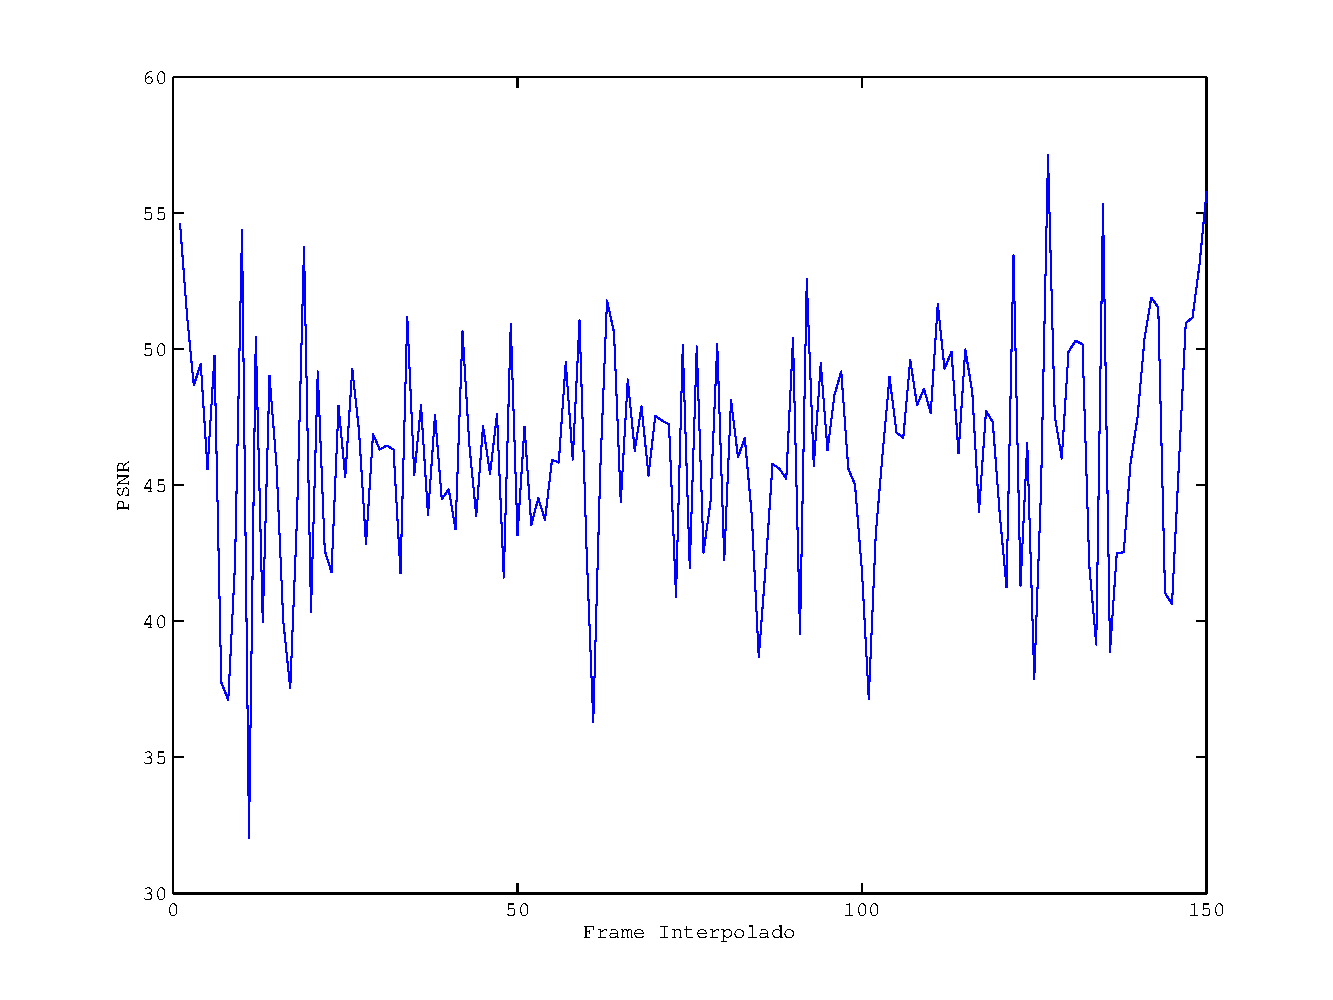
\includegraphics[width=.85\textwidth]{camara_fija-imagen_fija-lineal-psnr-k1.pdf}
    \caption{PSNR para 1 frame interpolado - M\'etodo Lineal}
    \label{fig:fija-fija_lineal-psnr-k1}
\end{figure}

\par De nuestro an\'alisis, entendemos que el error de interpolar entre frames
cercanos ser\'a similar, salvo cuando se tiene un cambio abruto de un frame al
siguiente en el video original. As\'i pues observamos en el gr\'afico (que es
similar a los de mayor cantidad de frames interpolados, salvo alguna
variaci\'on menor en los n\'umeros) que el PSNR\footnote{Recordemos que esta es
una m\'etrica que a mayor valor, m\'as fidedigna es la estimaci\'on del frame.}
se mantiene en valores por encima de los 45db la mayor parte del tiempo, salvo
ciertos picos de error que bajan su valor por unos pocos frames. Esto estar\'ia
relacionado con los cambios de iluminaci\'on distinguibles al ojo que tiene el
video.

\par Para finalizar con el an\'alisis del m\'etodo lineal para este video,
nuevamente generamos un video que comparase la diferencia entre los frames para
la interpolaci\'on lineal de 10 frames\footnote{\url{}} (utilizando el mismo
argumento que en splines, elegimos este par\'ametro ya que es el que mayor
desv\'io est\'andar tiene de todas las variantes). Presentamos a continuaci\'on
una captura del mismo, que consideramos representativa de las regiones de los
frames donde se influye m\'as en el error de interpolaci\'on.

\begin{figure}[H]
    \centering
    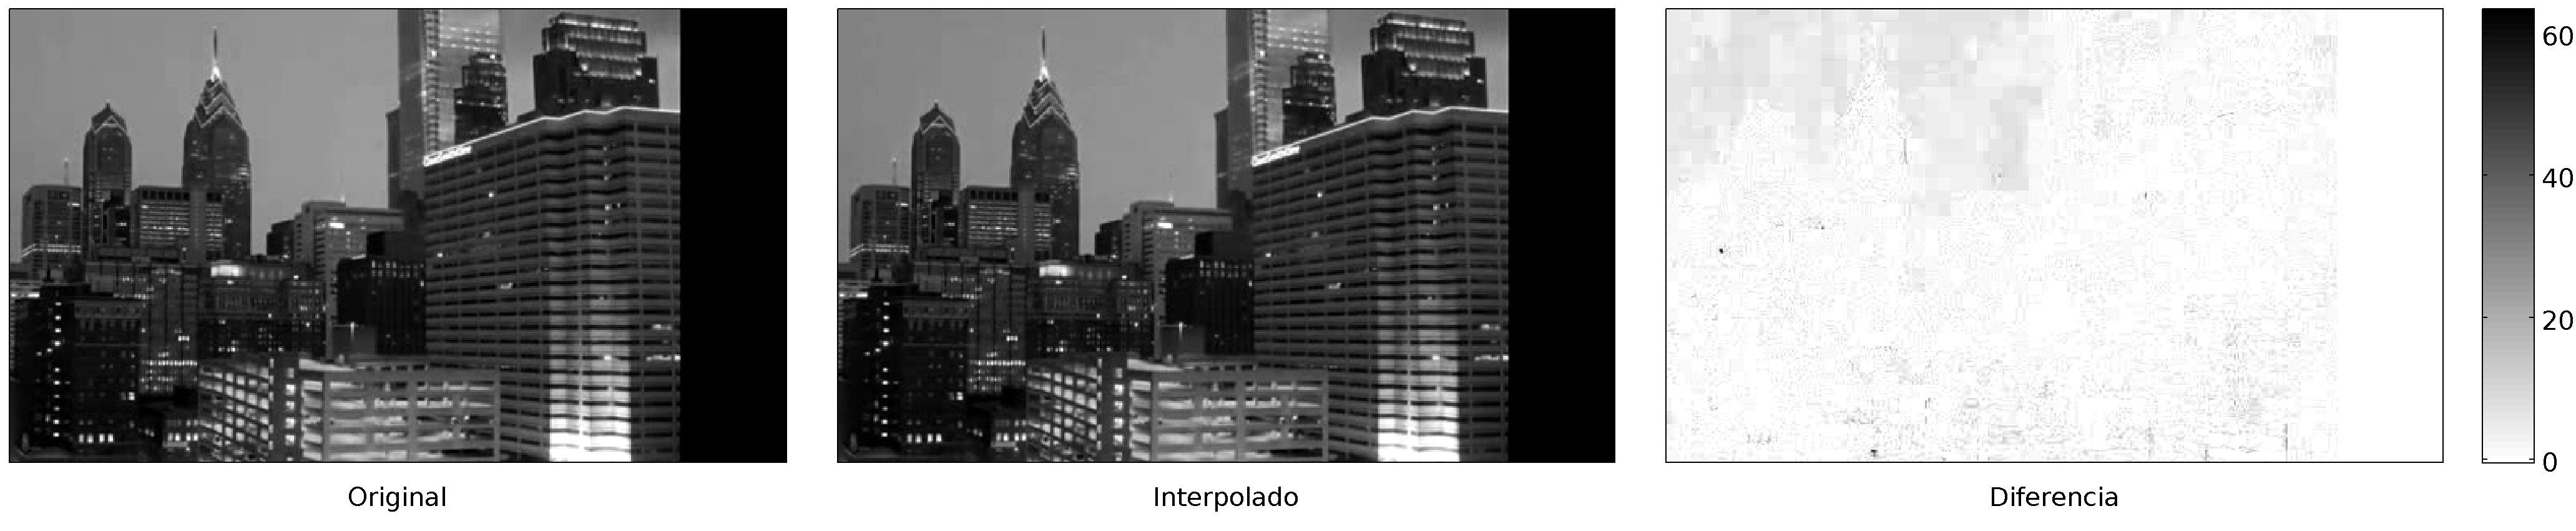
\includegraphics[width=\textwidth]{camara_fija-imagen_fija-lineal-k10.png}
    \label{fig:fija-fija_lineal-heatmap}
    \caption{Regi\'on peor aproximada por la interpolaci\'on lineal}
\end{figure}

\par El an\'alisis de este video comparativo, y las conclusiones, terminan
siendo exactamente igual que para el caso de splines de este mismo video. Se
puede observar como lo que afecta al error es la iluminaci\'on, y que las
partes m\'as afectadas por la misma (el cielo y las partes altas de los
edificios durante el d\'ia, y los sectores cercanos a las fuentes de luz
artificial durante la noche) son aquellas que mayor error (diferencia)
introducen. No queda mucho m\'as que agregar a lo ya dicho para el m\'etodo de
splines.

%---------------------------------------------------------------
\subsubsection{Vecino m\'as Cercano}
\par La metodolog\'ia de experimentaci\'on pare este m\'etodo no difiere
respecto de los 2 m\'etodos previos. As\'i pues, ahorrando explicaciones, se
pasa a exponer los resultados obtenidos de la experimentaci\'on.

\begin{figure}[H]
    \centering
    \subfloat[][Valor Medio]{
        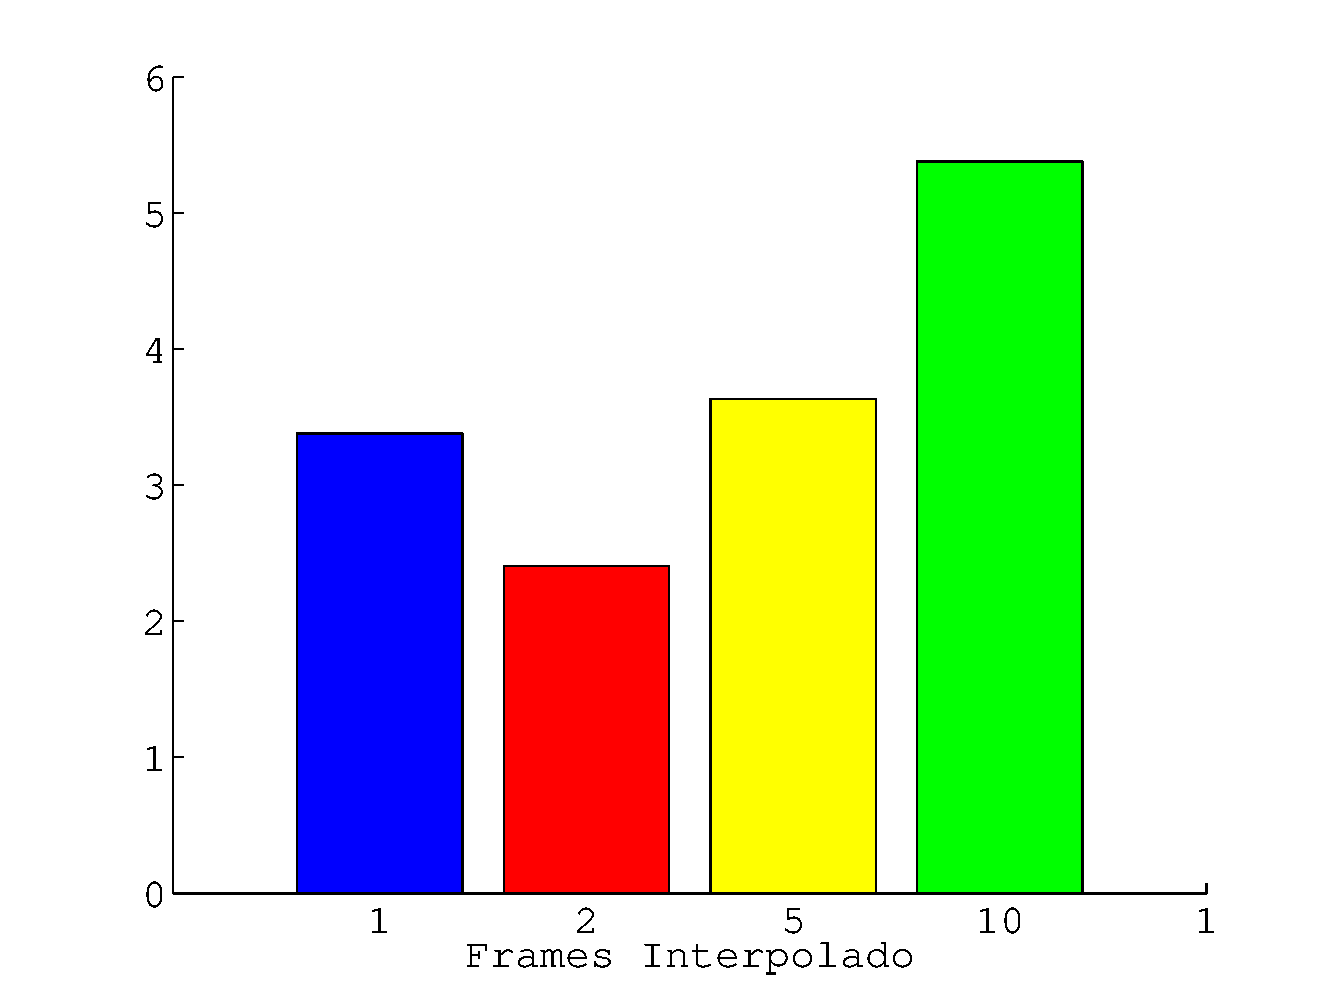
\includegraphics[width=.25\textwidth]{camara_fija-imagen_fija-mean_vecino.pdf}
    }%\hspace{20pt}
    \subfloat[][Desv\'io Est\'andar]{
        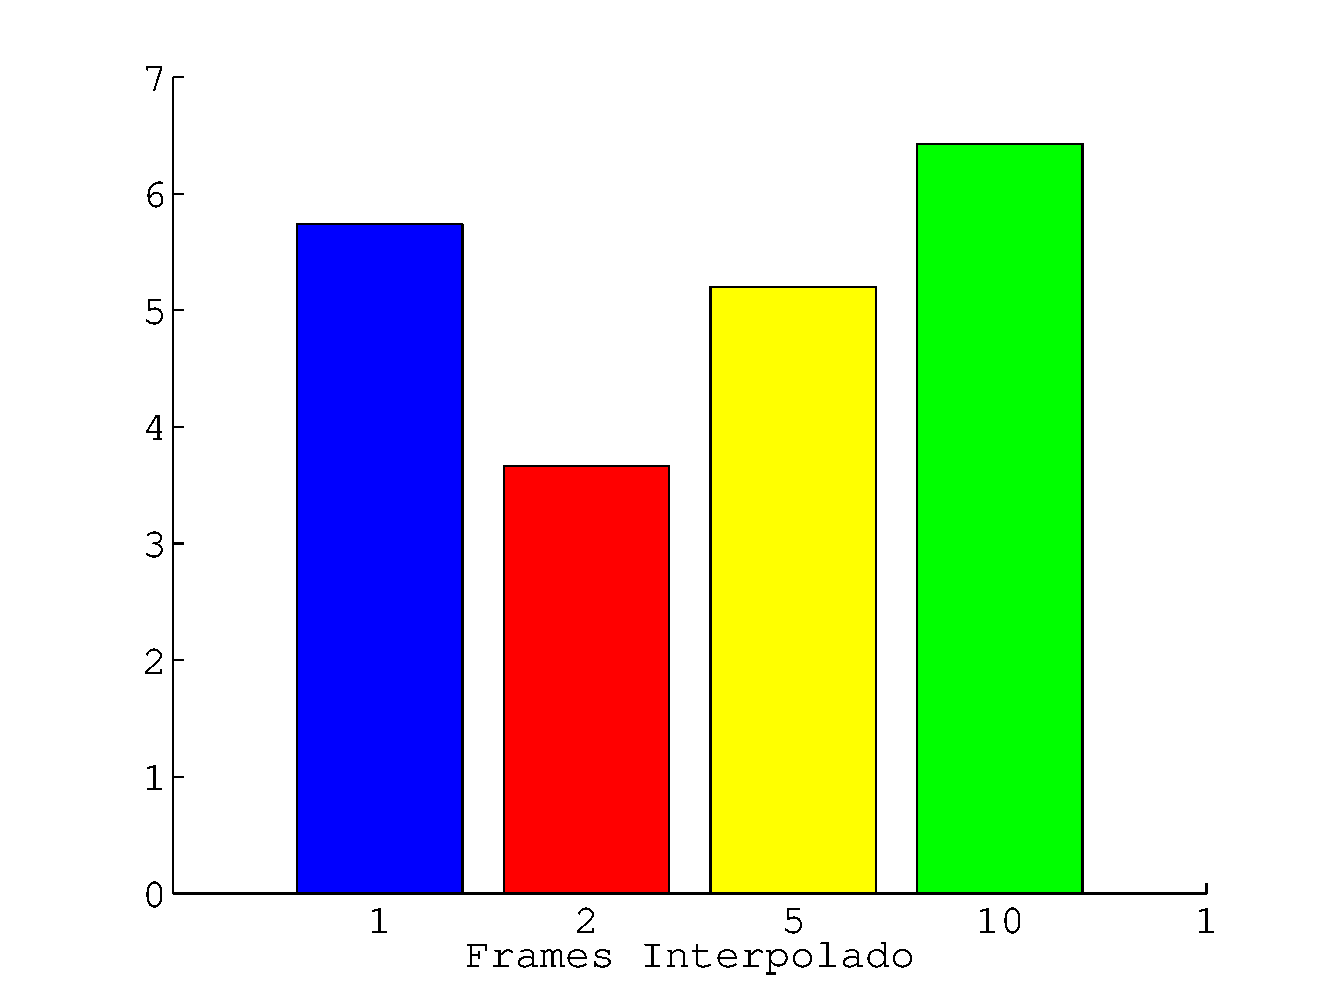
\includegraphics[width=.25\textwidth]{camara_fija-imagen_fija-std_vecino.pdf}
    }%\vspace{20pt}
    \subfloat[][M\'aximo]{
        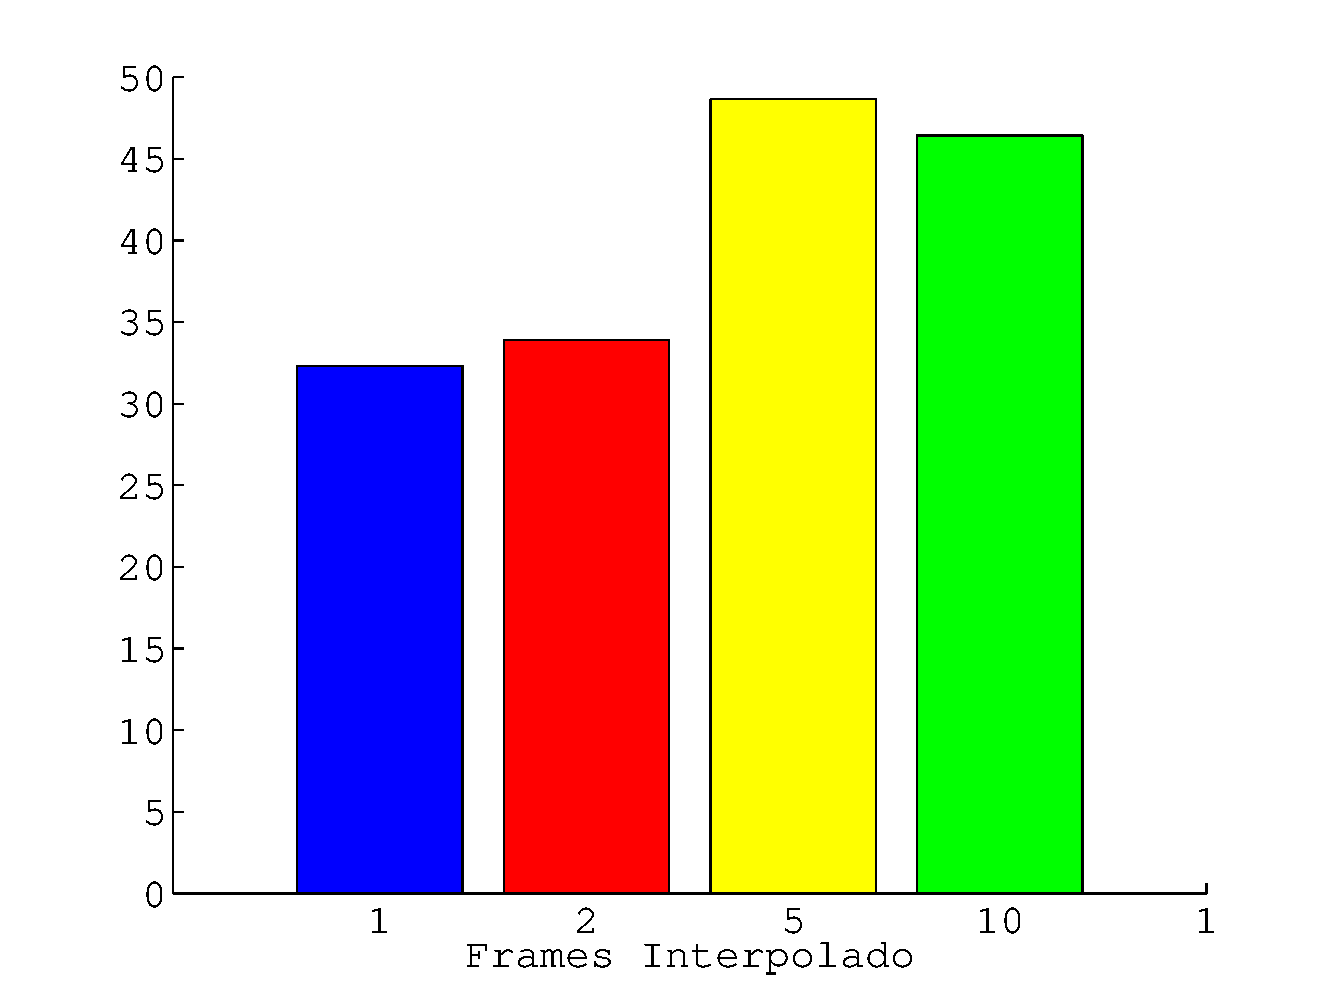
\includegraphics[width=.25\textwidth]{camara_fija-imagen_fija-max_vecino.pdf}
    }%\hspace{20pt}
    \subfloat[][M\'inimo]{
        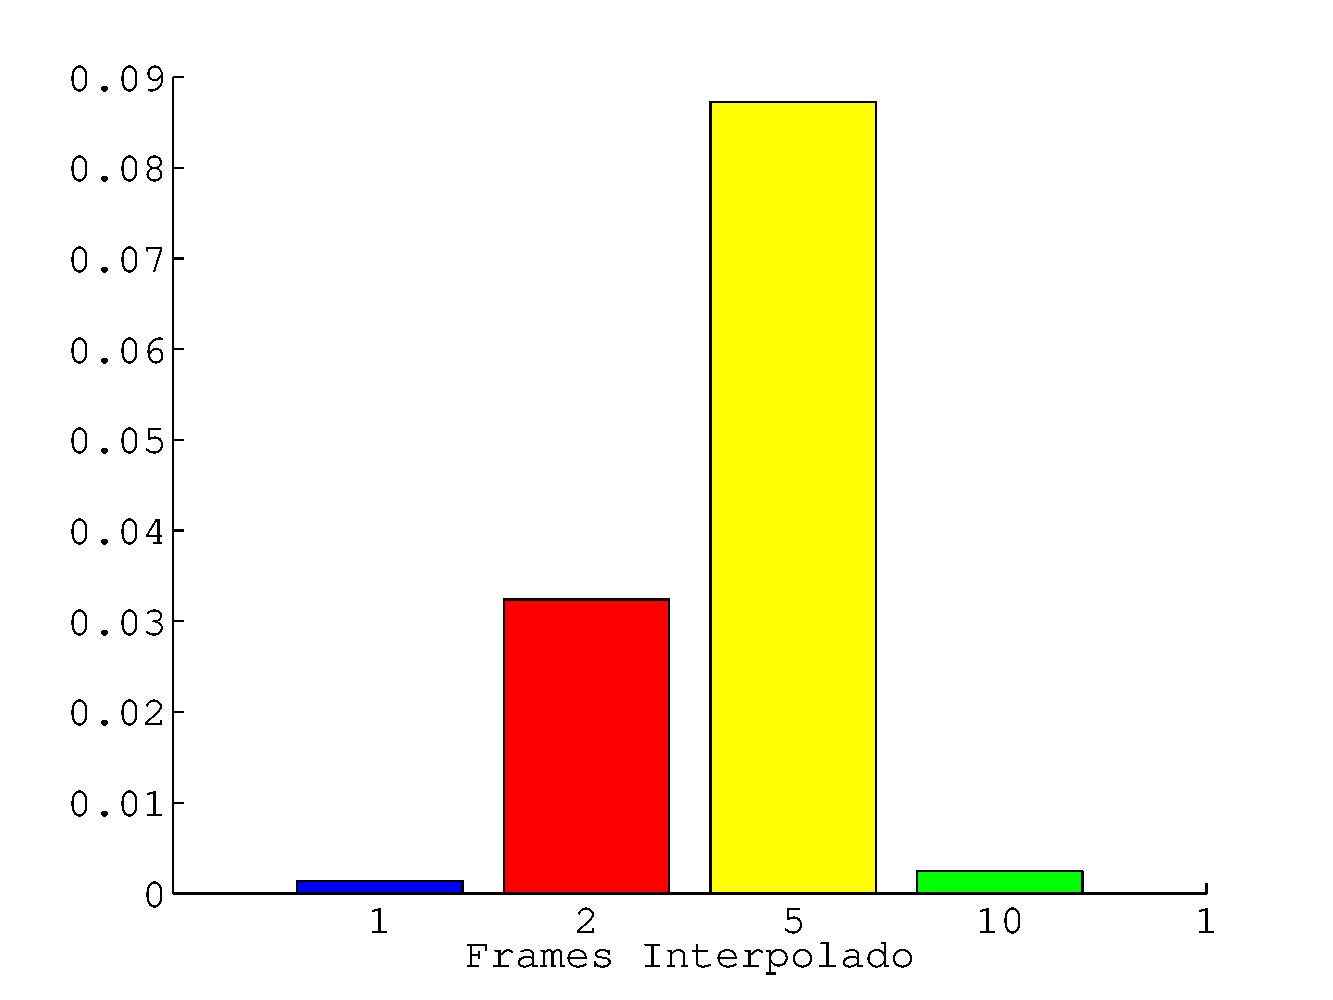
\includegraphics[width=.25\textwidth]{camara_fija-imagen_fija-min_vecino.pdf}
    }
    \caption{Est\'adisticas ECM Seg\'un Frames Interpolados - M\'etodo Vecino M\'as Cercano}
    \label{fig:fija-fija_vecino-mse_estadisticas}
\end{figure}

\par En los resultados expuestos en la figura \ref{fig:fija-fija_vecino-mse_estadisticas}
se encuentran relaciones entre las distintas variantes de frames interpolados, y
con n\'umeros bastantes cercanos tambi\'en, que al caso de splines. La diferencia
destacable radica en los valores de error m\'inimo alcanzado para las variantes de
interpolaci\'on de 1 y 10 frames, que como se puede observar son mucho m\'as chicos
que para los par\'ametros restantes. A\'un as\'i, una vista detallada de los valores nominales
nos muestra que a pesar de ser estos muy peque\~nos, ya se est\'a teniendo errores
m\'inimos de valor nominal muy peque\~no, haciendo que esta diferencia entre
distintas variantes del m\'etodo sean poco importantes. Es decir, tanto como si
se interpolan 1, 2, 5 o 10 frames, pareciera que siempre habr\'a alg\'un frame
interpolado con pr\'acticamente 0 error de estimaci\'on.

\par Respecto del an\'alisis del PSNR, y del video de comparaci\'on, los resultados
observados son exactamente id\'enticos a los explicados en el caso del m\'etodo
lineal para este video.

%\begin{figure}[H]
%    \centering
%    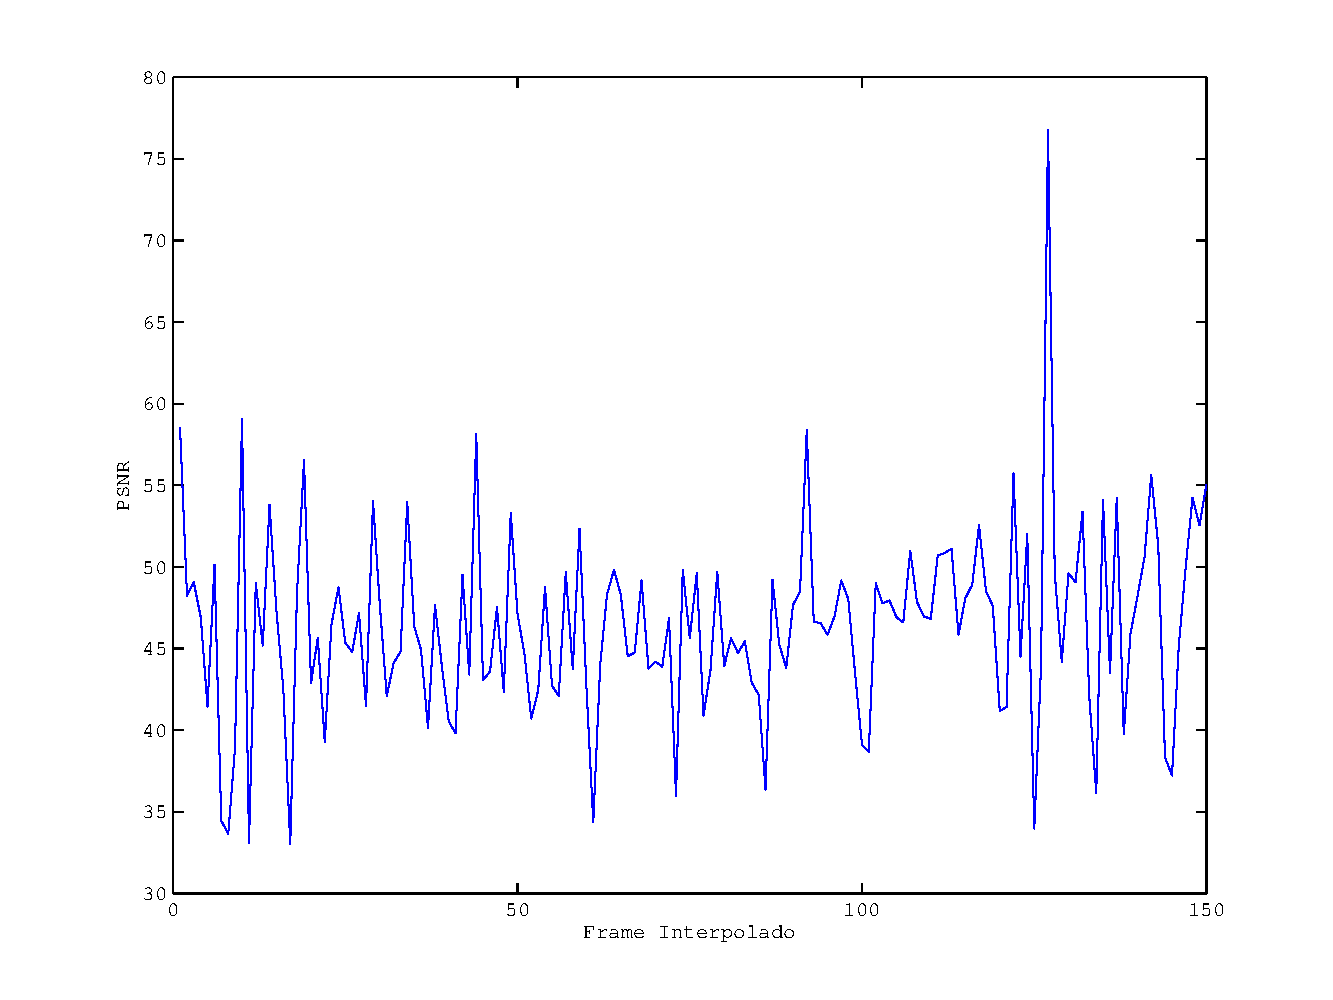
\includegraphics[width=.85\textwidth]{camara_fija-imagen_fija-vecino-psnr-k1.pdf}
%    \caption{PSNR para 1 frame interpolado - M\'etodo Vecino M\'as Cercano}
%    \label{fig:fija-fija_vecnio-psnr-k1}
%\end{figure}

%\begin{figure}[H]
%    \centering
%    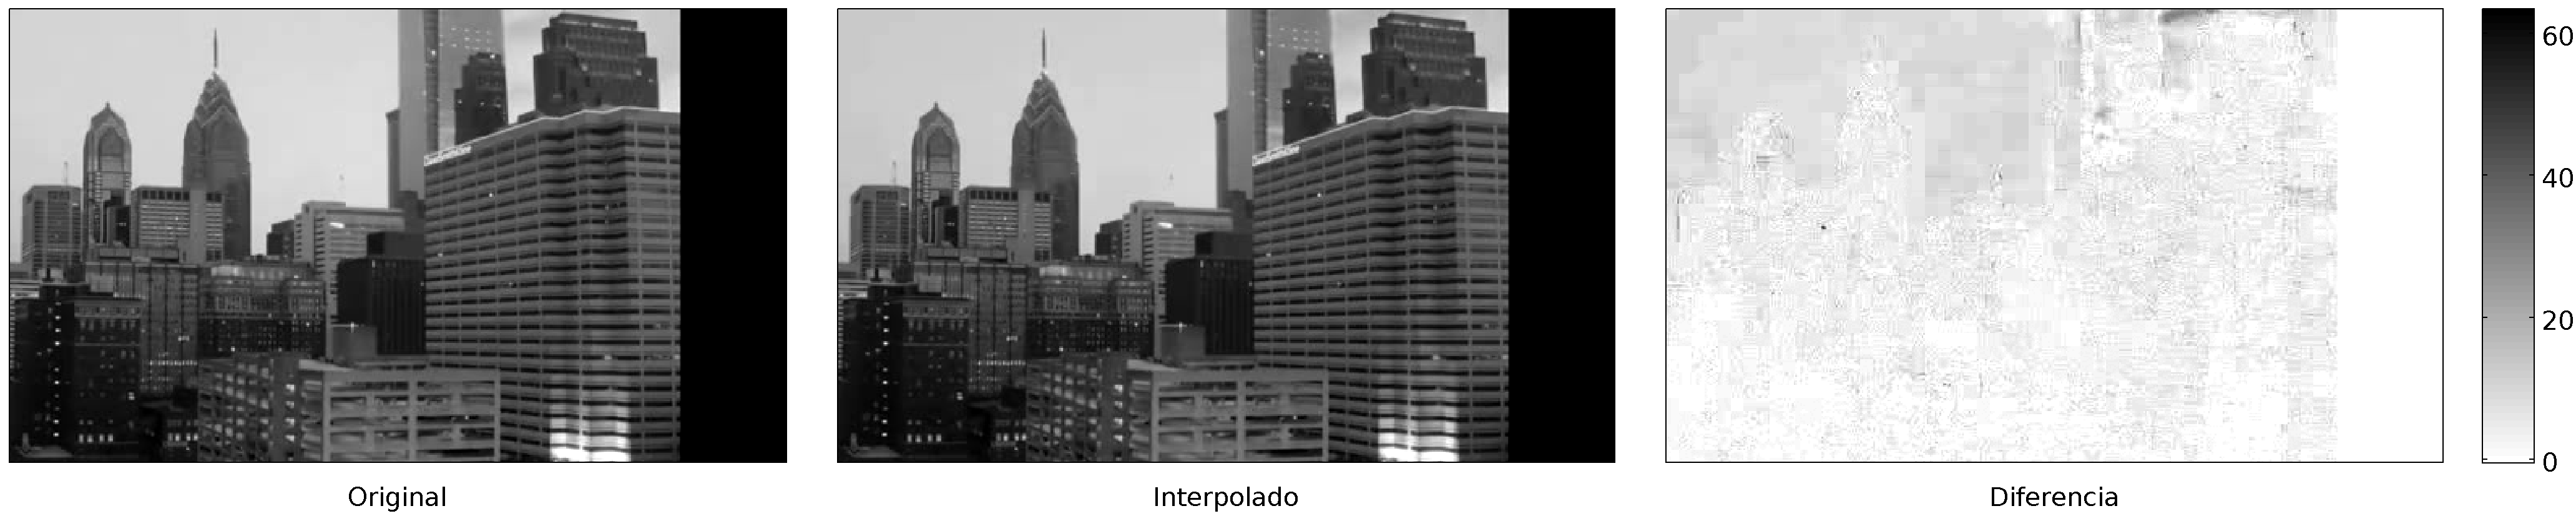
\includegraphics[width=\textwidth]{camara_fija-imagen_fija-vecino-k10.png}
%    \label{fig:fija-fija_vecino-heatmap}
%    \caption{Regi\'on peor aproximada por la interpolaci\'on del vecino m\'as cercano}
%\end{figure}

%---------------------------------------------------------------
\subsubsection{An\'alisis entre M\'etodos}
\par Luego de haber analizado cada m\'etodo independientemente de los dem\'as,
bas\'andonos \'unicamente en sus par\'ametros, pasamos a comparar cada m\'etodo
cualitativamente respecto de los otros, siempre para el mismo video.

\par En la figura \ref{fig:fija-fija_metodos} se puede observar el ECM y PSNR
frame a frame para el caso de 2 frames interpolados de c\'ada uno de los
m\'etodos.  En el caso del m\'etodo de splines, se expuso los resultados para
la interpolaci\'on del video completo (sin dividir por bloques), ya que como se
vi\'o en su respectivo an\'alisis, el comportamiento era similar no importa el
tama\~no del bloque.

\begin{figure}[H]
    \centering
    \subfloat[][ECM para 2 frames interpolados]{
        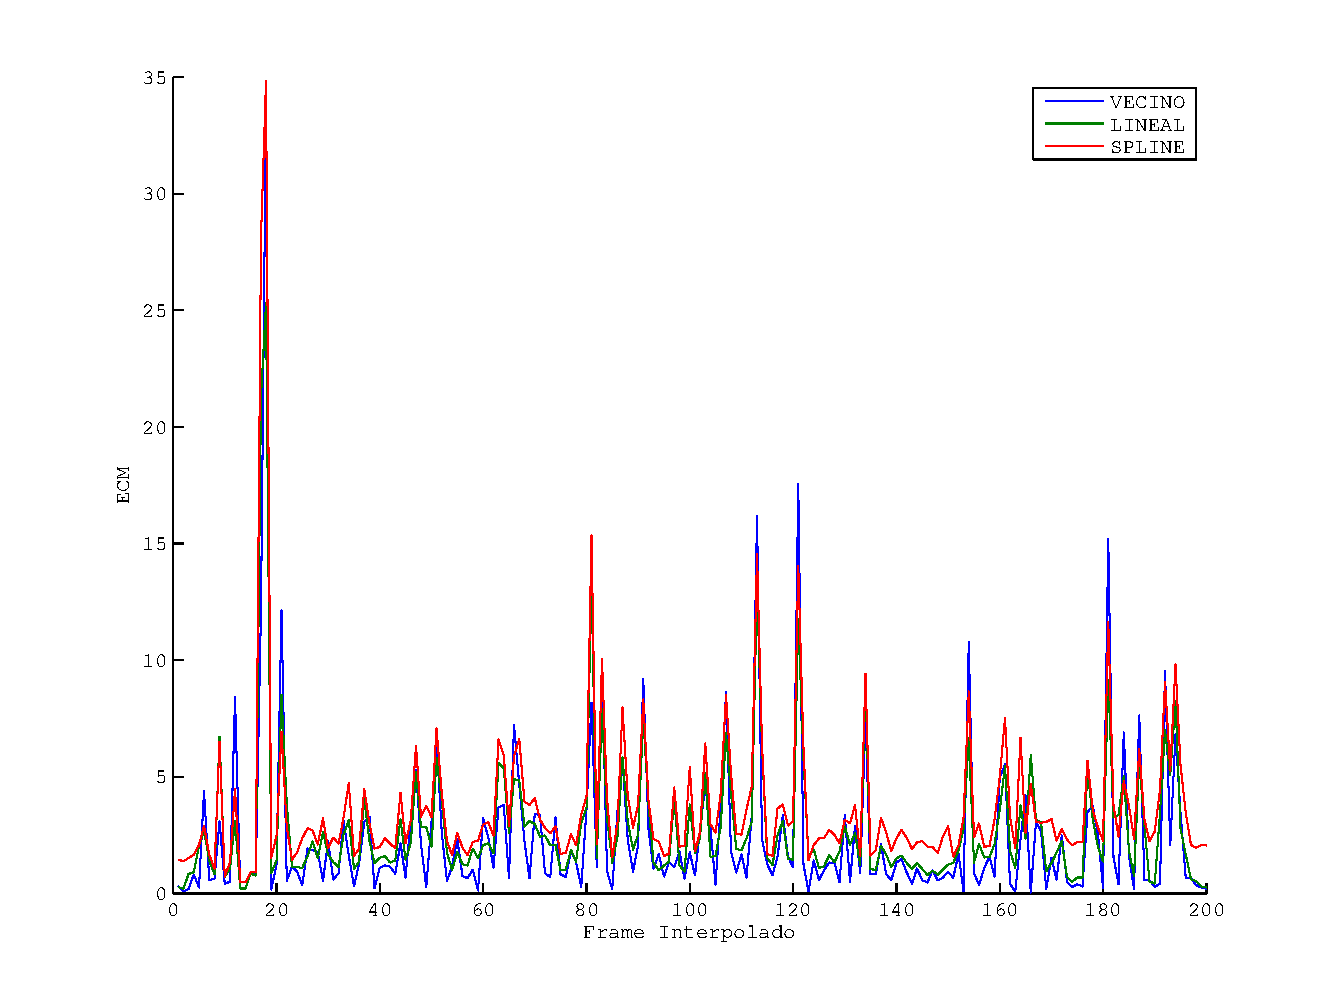
\includegraphics[width=.5\textwidth]{mse_methods-camara_fija-imagen_fija-k2.pdf}
        \label{subfig:fija-fija_mse-k2}
    }
    \subfloat[][PSNR para 2 frames interpolados]{
        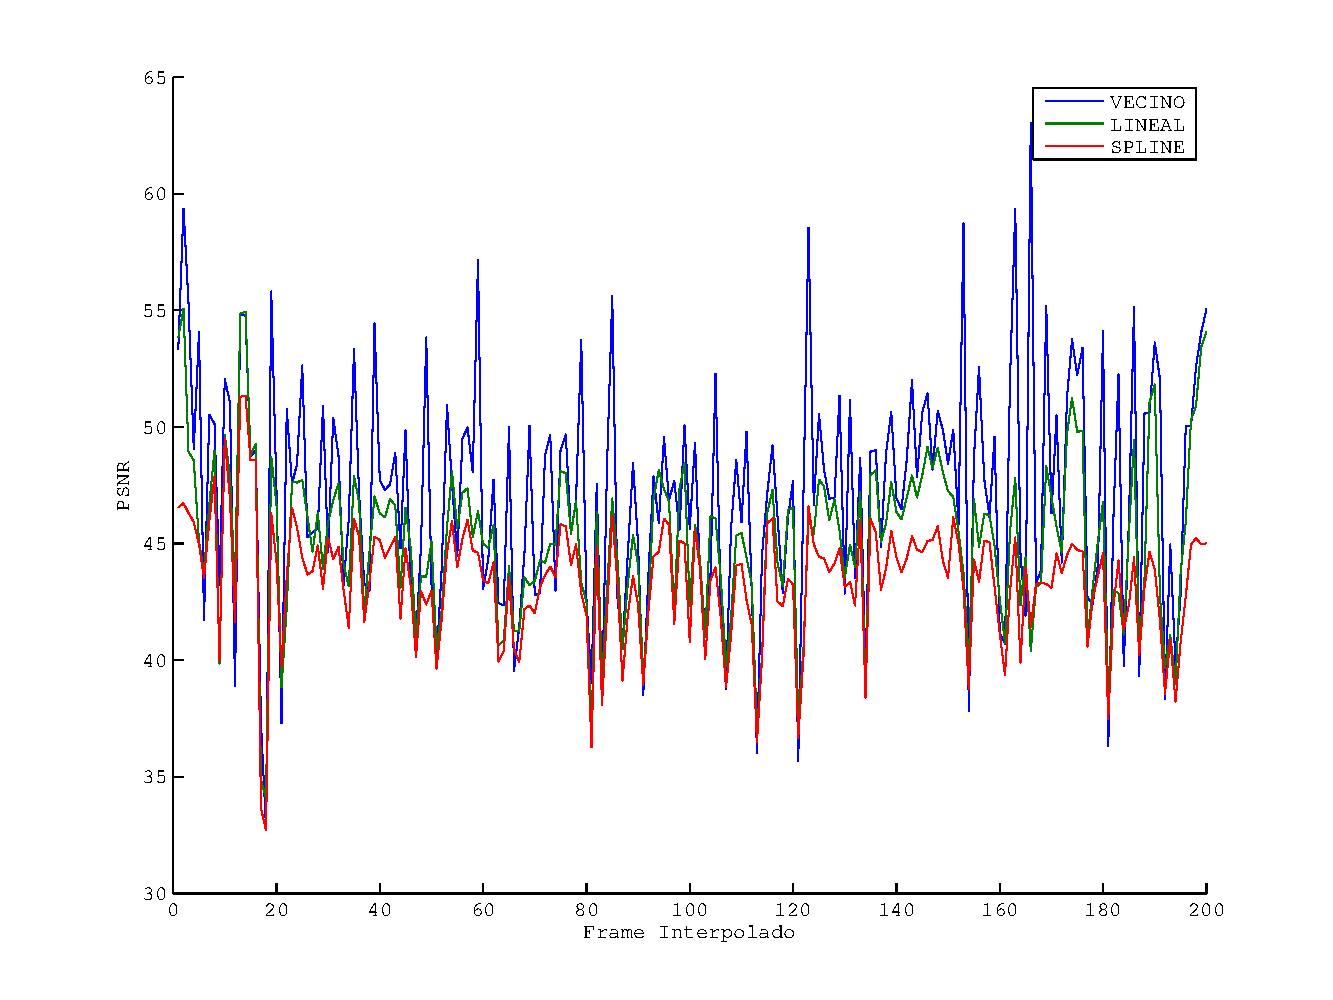
\includegraphics[width=.5\textwidth]{psnr_methods-camara_fija-imagen_fija-k2.pdf}
        \label{subfig:fija-fija_psnr-k2}
    }
    \caption{Comparativa de m\'etodos para 2 frames interpolados}
    \label{fig:fija-fija_metodos}
\end{figure}

\par En ambos gr\'aficos (aunque m\'as claramente en el PSNR) se observa un patr\'on
claro (m\'as all\'a de que haya frames que sean excepciones): la fidelidad es mejor
(o el error es menor) para el m\'etodo del vecino m\'as cercano, seguido por la
interpolaci\'on lineal y por \'ultimo el m\'etodo de splines.

\par No se exponen estas comparativas para otras variantes de interpolaci\'on,
ya que este patr\'on se repite en todos los casos. Adem\'as, vale la pena
recordar que para la cantidad de frames interpolados igual a 2 es para el cual
se obten\'ia el menor ECM medio para los m\'etodos de splines y vecino, y
virtualmente el menor tambi\'en para la interpolaci\'on lineal (la diferencia
para frames interpolados igual a 1 es m\'inima).

\par Pasemos a observar a continuaci\'on, las comparaciones para los valores
estad\'isticos del error cuadr\'atico medio:

\begin{figure}[H]
    \centering
    \subfloat[][Valor Medio]{
        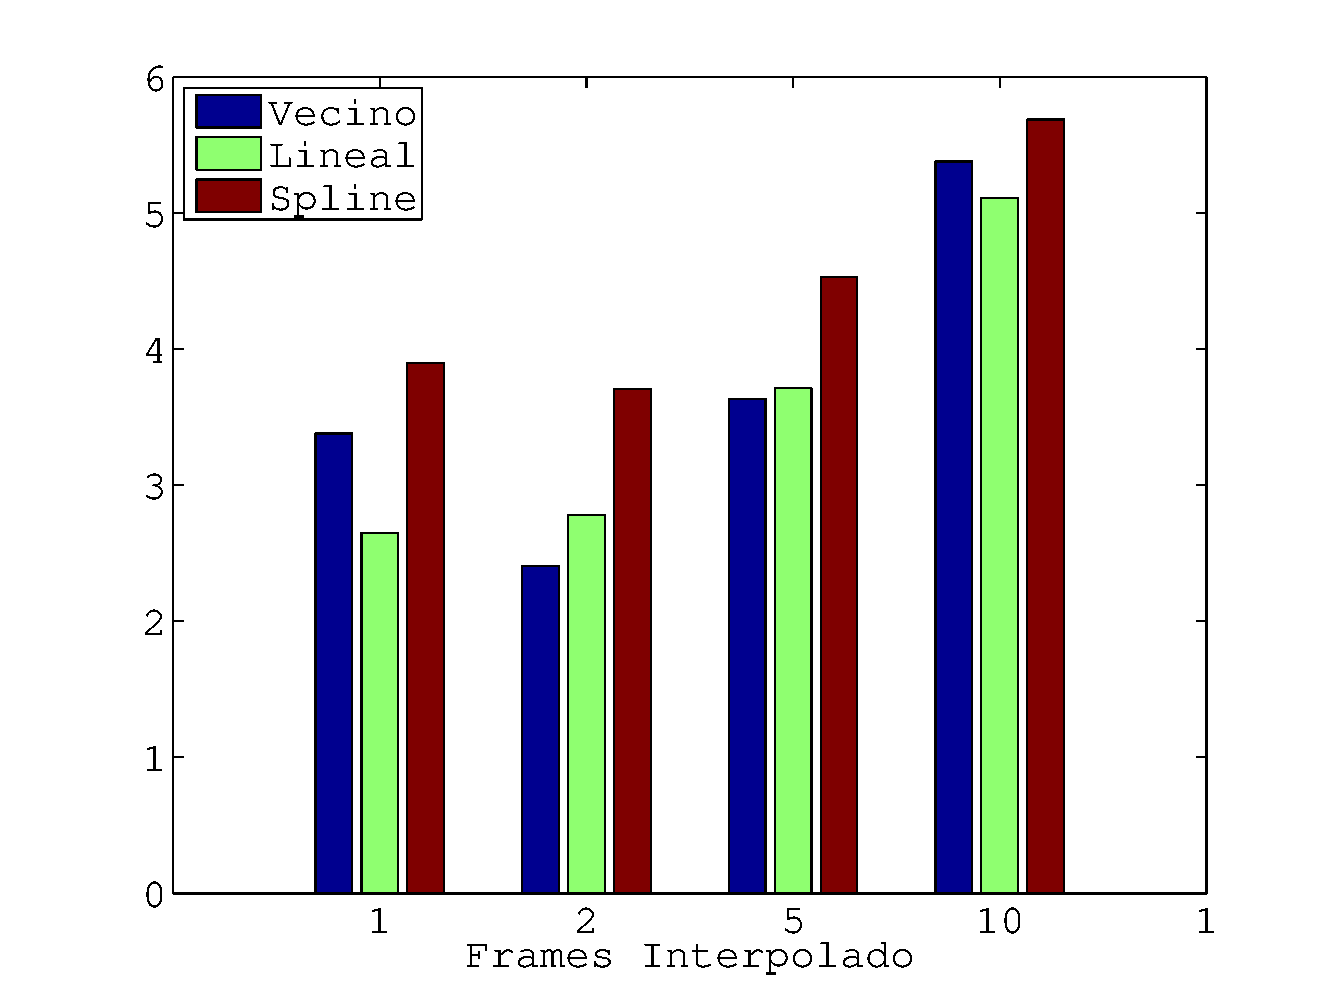
\includegraphics[width=.5\textwidth]{mean_methods-camara_fija-imagen_fija.pdf}
    }
    \subfloat[][Desv\'io Est\'andar]{
        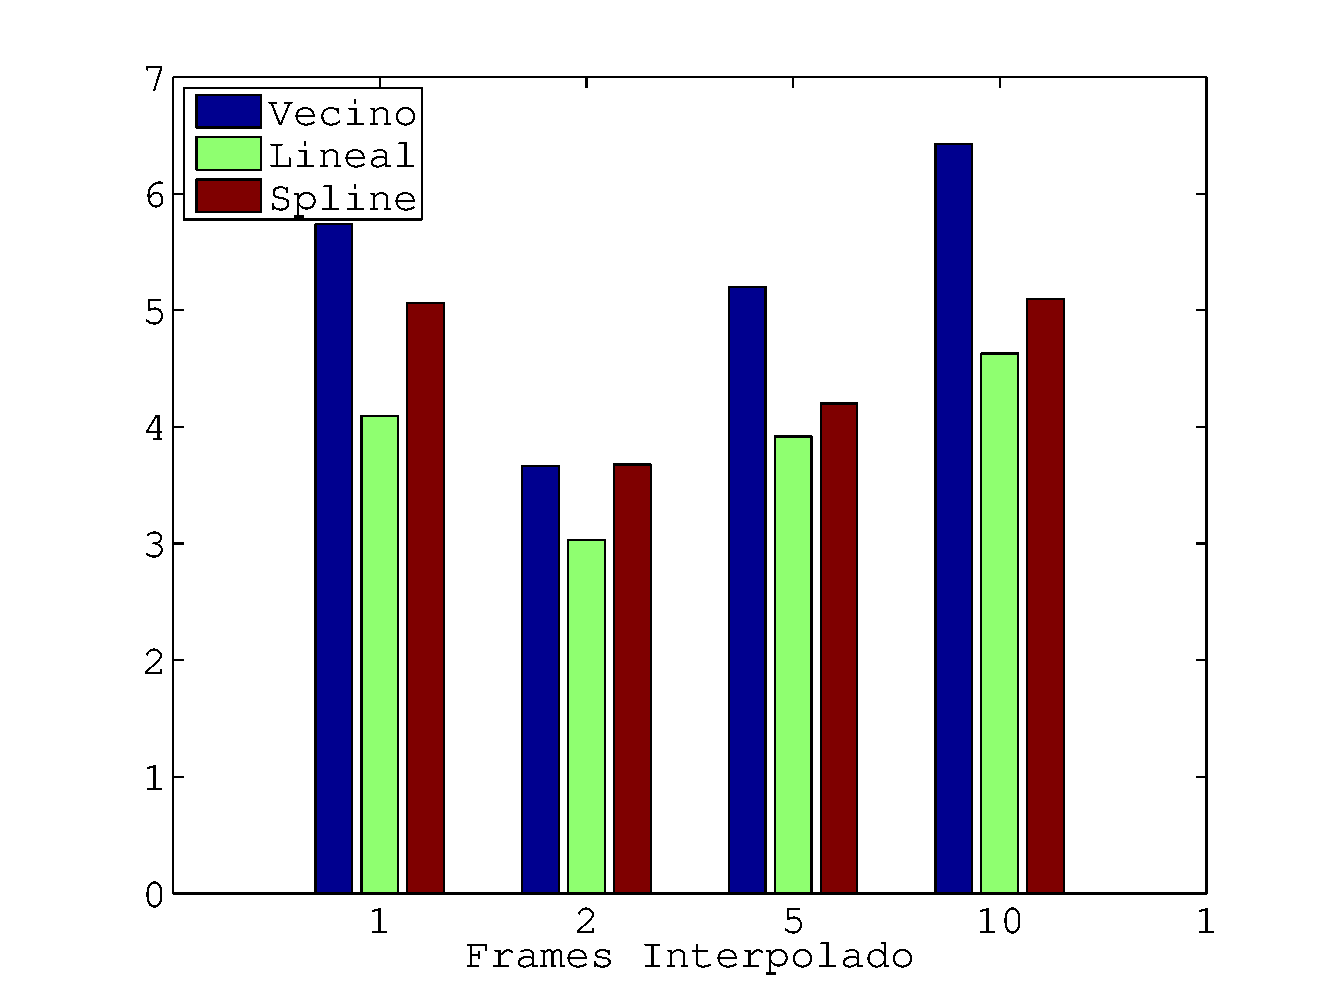
\includegraphics[width=.5\textwidth]{std_methods-camara_fija-imagen_fija.pdf}
    }\\
    \subfloat[][M\'aximo]{
        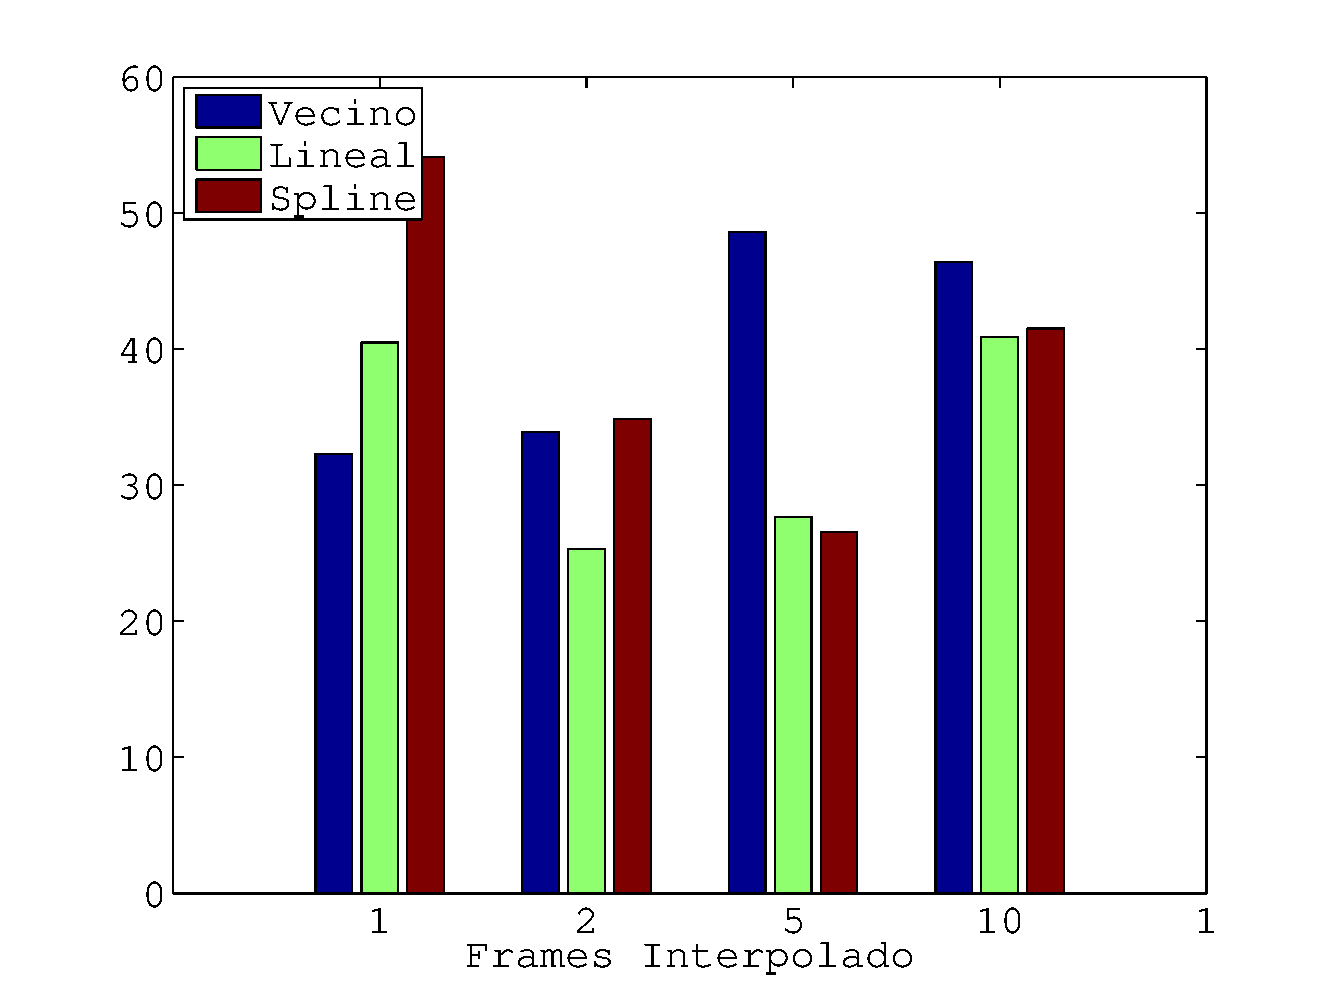
\includegraphics[width=.5\textwidth]{max_methods-camara_fija-imagen_fija.pdf}
    }
    \subfloat[][M\'inimo]{
        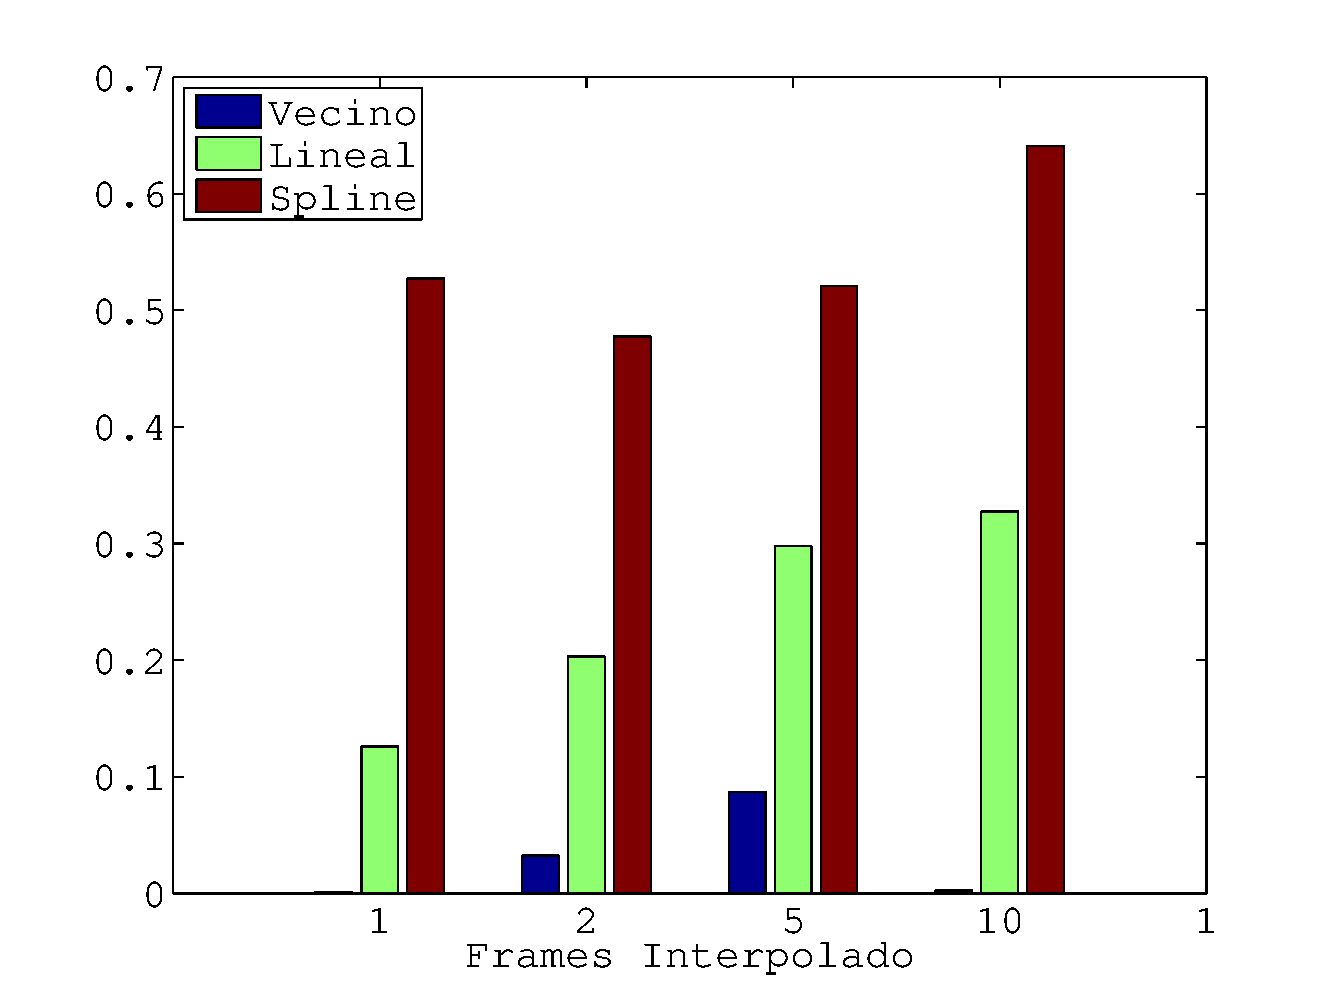
\includegraphics[width=.5\textwidth]{min_methods-camara_fija-imagen_fija.pdf}
    }
    \caption{Est\'adisticas ECM - Comparativa de M\'etodos}
    \label{fig:fija-fija_methods-mse_estadisticas}
\end{figure}

\par Al observarse estos datos, aparece algo que \emph{a priori} parecer\'ia
una contradicci\'on: el valor medio del ECM para el m\'etodo lineal es menor en
2 de las variantes (cantidad de frames 1 y 10) que el m\'etodo del vecino m\'as
cercano. Analizando un poco esto (pues, como afirmamos unos p\'arrafos m\'as
arriba, para todas las variantes encontramos que el PSNR para el m\'etodo del
vecino m\'as cercano segu\'ia el patr\'o de ser m\'as alto que el de los
restantes m\'etodos), entendemos que el motivo de esto se debe a que el
m\'etodo del vecino tiene picos m\'as amplios donde comete mucho m\'as error
que el m\'etodo de interpolaci\'on lineal. Esto puede observarse, nuevamente,
en la figura \ref{fig:fija-fija_metodos}.  Esto explica el porque del valor
medio del error es m\'as bajo para el m\'etodo lineal, aunque en la gran
mayor\'ia de los frames la aproximaci\'on del m\'etodo del vecino es mejor.

%---------------------------------------------------------------
\subsubsection{Conclusiones}
\par A lo largo de la experimentaci\'on para el tipo de video
\emph{c\'amara-fija, im\'agen fija}, observamos que todos los m\'etodos
mostraron un buen comportamiento.  Esta afirmaci\'on es subjetiva y basada en
la opini\'on de los autores luego de observar los videos resultantes. Para el
ojo humano, las diferencias entre los m\'etodos (o para el mismo m\'etodo con
diferentes par\'ametros) fueron imperceptibles.

\par A\'un as\'i, un an\'alisis m\'as objetivo basado en las m\'etricas nos
lleg\'o a indicar que, al menos para los par\'ametros evaluados, el m\'etodo
del vecino pareciera ser mejor, incluso cuando se interpolan muchos frames
(recordemos que una las hip\'otesis al comienzo de la experimentaci\'on era que
los m\'etodos de spline e interpolaci\'on lineal deber\'ian ser mejores en caso
de tener que estimar/reconstruir muchos frames). Si bien su ECM medio es m\'as
alto que el de otros m\'etodos, pudimos observar que tambi\'en lo es su
desv\'io est\'andar. Y justamente esto \'ultimo es lo que nos permiti\'o
descubrir que el motivo de su ECM medio m\'as alto se debe a que, en
determinados frames (los m\'as alejados de los 2 frames utilizados para
interpolar, de hecho) el m\'etodo tiene un error m\'as alto que el resto. Como
esto \'ultimo ocurre seguido, el ECM tiende a subir, pero al observar el PSNR
frame a frame se pudo concluir que en realidad, para la gran mayor\'ia de los
frames interpolados, el m\'etodo del vecino superaba a sus pares.

\par Esto \'ultimo no es un resultado menor, m\'as si se tiene en cuenta que
el m\'etodo del vecino es el m\'as barato computacionalmente hablando, como ya
se ha visto.

\par En otra l\'inea de an\'alisis, tambi\'en se observ\'o que al menos para
este tipo de video, que el tama\~no de bloque utilizado no hizo variar a la
efectividad del m\'etodo de spline. Esto, si bien no esperado al comenzar los
experimentos, es razonable si se considera que en si mismo el video no presenta
casi cambios, m\'as all\'a del brillo de sus puntos debido al cambio de
iluminaci\'on. Tiene sentido entonces que el resultado de splines no var\'ie ya
que ''la funci\'on interpolada''\footnote{Los pixels a lo largo de los frames.}
camb\'ian en funci\'on del frame de manera ''suave'', con lo cual no importe
desde que frame a que frame se genere el spline, sus valores en los extremos de
los bloques tender\'ian a ser similiares a lo que se les exije en el m\'etodo a
los \emph{sub-splines}.

\par Para finalizar este experimento, vale la pena remarcar nuevamente que si
bien la interpolaci\'on de todos los m\'etodos tuvieron error, el mismo siempre
fue muy peque\~no nominalmente. De hecho, como se mencion\'o al principio de
estas conclusiones, fueron imperceptibles para los autores. Si se observan los
errores m\'aximos obtenidos de todos los m\'etodos, observamos que el error
m\'as grosero cometido fue de 60, el cual quedar\'a en evidencia que es un
valor peque\~no al compararlo con los errores de los m\'etodos en los otros
tipos de videos que se exponen m\'as adelante. M\'as a\'un, si se observar los
videos comparativos de las interpolaciones, se observar\'a que el \emph{heatmap}
de la diferencia absoluta entre el frame original y el interpolado nunca tiene
regiones enteras con mucho (o incluso, m\'as que poco) error. A lo sumo existen
peque\~nos grupos de no m\'as de 10 p\'ixeles que muestran un error alto, pero
nunca regiones.

%---------------------------------------------------------------


%---------------------------------------------------------------
\newpage
\subsection{C\'amara Fija - Im\'agen M\'ovil}
\IEEEPARstart{A}{}

%---------------------------------------------------------------
\subsubsection{Splines}

%---------------------------------------------------------------
\subsubsection{Lineal}

%---------------------------------------------------------------
\subsubsection{Vecino}

%---------------------------------------------------------------
\subsubsection{M\'etodos}

%---------------------------------------------------------------
\subsubsection{Conclusiones}

%---------------------------------------------------------------


%---------------------------------------------------------------
\newpage
\subsection{C\'amara M\'ovil - Im\'agen Fija}

%---------------------------------------------------------------
\newpage
\subsection{C\'amara M\'ovil - Im\'agen M\'ovil}

%---------------------------------------------------------------
\newpage
\subsection{An\'alisis por M\'etodo en funci\'on del Video}

%---------------------------------------------------------------
\newpage
\subsection{Artifacts}
En este contexto, consideraremos \emph{artifacts} a aquellos errores visuales resultantes de la aplicaci\'on de un m\'etodo o t\'ecnica. En particular a aquellos que no reflejan una situación verosímil en la vida real\footnote{Esto es muy subjetivo, pero no me explayo mas porque bordea la filosofía.}\footnote{Por ejemplo la pierna fantasma de la slide de la presentación del tp.}.

Dividiremos nuestro análisis en diferentes casos, en función de las siguientes variables:
\begin{itemize}
	\item Método utilizado para la interpolación
	\item Tipo Movimiento grabado por la Cámara
	\item Tipo de Movimiento de la Cámara
	\item En el caso de splines, se considera además el tamaño del bloque utilizado
\end{itemize}

Los algoritmos utilizados para producir el efecto de cámara lenta pueden clasificarse en los siguientes tipos:
\begin{itemize}
	\item Métodos predictivos: Interpolación polinomial de frames intermedios, intenta \emph{llenar los huecos} de forma natural entre cada par de frames, intentando predecir el comportamiento del video entre 2 frames conocidos.
	\item Métodos no predictivos: Por ejemplo, vecino mas cercano, se limita a copiar frames, sin interés en generar nueva información.
\end{itemize}

\subsection{Interpolación por vecino mas cercano}
Dado que este método de \emph{slowmotion} es un método \emph{no predictivo} no se producirán artifacts bajo nuestra definición, simplemente el video ralentizado tendrá un efecto de \texttt{lag} en donde la reproducción parece trabada. Esto es esperable, ya que este método copia frames consecutivamente para lograr un efecto de mayor tiempo de visualización por frame en la reproducción en tiempo real. 

\subsection{Interpolación lineal}
\subsubsection{Cámara fija e imagen fija - Caso de laboratorio}
En nuestro caso de laboratorio \footnote{Un video conteniendo un único frame repetido muchas veces.} puede observarse que al ser todos los pares de frames iguales los frames interpolados linealmente también lo serán ya que la recta que une a todos los píxeles entre los 2 frames consecutivos es una constante. No se observan artifacts.

\subsubsection{Cámara fija e imagen fija}
Consideremos en este caso, un video de un objeto inmóvil, pero con cambios de iluminación. Lo que observamos es, que a medida que vamos aumentando el factor de ralentización \footnote{Agregando mas frames intermedios mediante interpolación.} se van suavizando los cambios en el video. Puntualmente, en el video original, observamos el suave cambio de color del cielo y el rápido encendido y apagado de luces. En el video ralentizado, mientras más frames fueron agregados artificialmente, se produce un efecto de suavizamiento de estos cambios rápidos, dándoles una sensación de transición lenta entre encendido y apagado de luces. Respecto a los cambios lentos, no observamos nada muy evidente.

\subsubsection{Cámara fija e imagen móvil}
En este caso, se considera una cámara en posición fija, captando una escena con mucho movimiento y fondo estático. Particularmente es una escena de un partido de fútbol. Puede observarse que al aumentar el factor de slowmotion, se observa un efecto de \texttt{fantasmeo} en la parte móvil de la escena. Esto puede explicarse desde un punto de vista de la clasificación en métodos predictivos. Bajo el objetivo de construir una secuencia verosímil de frames entre dos frames consecutivos\footnote{\url{https://en.wikipedia.org/wiki/Motion_estimation} . En nuestro caso simplemente los \texttt{motion vectors} mapean idénticamente los píxeles entre dos frames consecutivos.}, intenta predecir el movimiento de los objetos presentes, mientras menos distancia se mueva el objeto entre par de frames originales, mas acertada será esta predicción. Por otro lado, al estar mapeando los píxeles idénticamente al predecir el movimiento, nos queda esta sensación de fantasmeo, producida por la transición suave entre los colores en la región donde se produce el movimiento. Otro buen ejemplo donde se ve esta anomalía es la figura \ref{fig:lineal}, corrida sobre el video \emph{city.avi}. Respecto al fondo estático, al ser los valores de los píxeles iguales entre frames, la recta que los une también es constante y dichos píxeles son copiados idénticamente en cada frame agregado.

\subsubsection{Cámara móvil e imagen fija}
En este caso lo que se observa es algo similar a lo mencionado anteriormente de \emph{motion prediction}, al moverse la figura, particularmente en los bordes de la misma, donde la diferencia entre el gris de la figura y el fondo negro es mas visible, se producen artifacts de fantasmeo mas marcado, nuevamente esto es producido por nuestro mapeo idéntico de píxeles entre frames, produciendo una transición suave de colores en las regiones donde se producen los cambios mas bruscos. El fondo no presenta artifacts evidentes. Como detalle, notar que en la parte frontal central del robot, los artifacts son mas leves, asumimos que esto se debe a que a pesar de mapear idénticamente los píxeles, la varianza de color de la región es muy baja.

\subsubsection{Cámara móvil e imagen móvil}
Este caso de prueba se caracteriza por rápidos cambios en los ángulos de la filmación y por una escena rápida ocurriendo de fondo. Probablemente este sea el peor caso, cualitativamente hablando. Lo que se observa es que a medida que se aumenta el factor de ralentización, el video reconstruido sufre mucho más el hecho de predecir el movimiento con un mapeo idéntico de píxeles entre frames. Casi que para valores altos de ralentización es casi imposible de seguir el movimiento correcto ya que aparecen cosas que al ojo humano le parecerían dobles figuras\footnote{Por ejemplo cuando la pelota y la cámara se mueven al mismo tiempo, parece que hay varias pelotas.}

\subsubsection{Transición rápida de blanco a negro}
Mas allá del fantasmeo producido por la predicción del movimiento errónea, los cambios rápidos de blanco a negro, agregan un, si se quiere, natural degradé entre blanco y negro pasando por gris. Sin embargo, en la realidad, esto no necesariamente ocurre. Este método agrega un efecto espurio a al reacción química mostrada en el video.

% --------------- Splines ------------------

\subsection{Interpolación cúbica con splines}
\subsubsection{Cámara fija e imagen fija - Caso de laboratorio}

\subsubsection{Cámara fija e imagen fija}

\subsubsection{Cámara fija e imagen móvil}

\subsubsection{Cámara móvil e imagen fija}

\subsubsection{Cámara móvil e imagen móvil}

\subsubsection{Transición rápida de blanco a negro}



%---------------------------------------------------------------
\newpage
\subsection*{Experimentos a Futuro}
